\section{Homotopy Groups}

\subsection{Homotopy}
We follow chapter 14 of \cite{Bredon} for this subsection.\\

To start of, we recall the basic definitions of homotopies.

\begin{definition}[Homotopy]
    Two maps $f_0, f_1 \colon X \to Y$ are said to
    be \textit{homotopic} if there exists a homotopy
    $F \colon X \times I \to Y$ such that
    $F(x,0) = f_0(x)$ and $F(x,1) = f_1(x)$ for
    all $x \in X$.
\end{definition}

\begin{definition}[Homotopy equivalence]
    A map $f \colon X \to Y$ is said to be a \textit{homotopy
    equivalence} if it is an isomorphism in
    $\hTop$.
\end{definition}

\begin{lemma}[Reparametrization Lemma]
    Let $\varphi_1, \varphi_2$ be maps
    $\left( I, \partial I \right) \to 
    \left( I, \partial I \right) $ which are equal on
    $\partial I$. Let
    $F \colon X \times I \to Y$ be a homotopy and let
    $G_i (x,t) = F\left( x, \varphi_i(t) \right) $ for
    $i = 1,2$. Then $G_1 \simeq G_2 \rel
    X \times \partial I$.
\end{lemma}

We shall use $c$ to denote the constant homotopy.

\begin{proposition}[]
    $F * c \simeq F \rel X \times \partial I$ and
    $c * F \simeq F \rel X \times \partial I$.
\end{proposition}

\begin{definition}[]
    If $F \colon X \times I \to Y$ is a homotopy, then we
    define $F^{-1} \colon X \times I \to Y$ by
    $F^{-1}\left( x,t \right) = F(x,1-t)$. 
\end{definition}

Note that $F^{-1}$ is precisely the inverse
to $F$ in $\hTop$.

\begin{proposition}[]
    For any homotopies $F,G,H$ for which the
    concatenations 
     are defined, we have
     \[
         \left( F * G  \right) * H
         \simeq F * \left( G * H \right) 
         \rel X \times \partial I.
     \] 
\end{proposition}


\begin{proposition}[]
    For homotopies $F_1, F_2, G_1, G_2$,
    if $F_1 \simeq F_2 \rel X \times \partial I$ and
    $G_1 \simeq G_2 \rel X \times \partial I$, then
    $F_1 * G_1 \simeq F_2 * G_2 \rel X \times \partial I$.
\end{proposition}

Note that all of the discussion of concatenation of
homotopies goes through with no difficulties for the cases
in which all homotopies are relative to some subspace
$A \subset X$ or are homotopies of pairs
$\left( X, A  \right) \to \left( Y, B \right) $.\\
It follows that homotopy between maps of
pairs $\left( X,A \right) \to \left( Y,B \right) $ is
an equivalence relation. The set of homotopy classes
of these maps is commonly denoted by
$\left[ X,A ; Y ,B \right] $ or just
$\left[ X;Y \right] $ if $A = \varnothing$.

\begin{theorem}[]\label{Thm:299221}
    If $f_0 \simeq f_1 \colon X \to Y$ then
    $M_{f_0} \simeq M_{f_1} \rel
    X + Y$ and
    $C_{f_0} \simeq C_{f_1} \rel
    Y + \text{vertex}$.
\end{theorem}


To show this, one needs the following basic topological
proposition:
\begin{proposition}[] \label{prop:92031999}
    If $f \colon X \to Y$ is a quotient map and
    $K$ is locally compact Hausdorff, then
    $f \times 1 \colon X \times K \to Y \times K$ is
    a quotient map.
\end{proposition}

\begin{proof}[Proof of Theorem \ref{Thm:299221}]
    First, let $F \colon X \times I \to Y$ be the homotopy
    between $f_0$ and $f_1$. Now define $h \colon
    M_{f_0} \to M_{f_1}$ by $h(y) = y$ for
    $y \in Y$ and
    \[
    h\left( x,t \right) = 
    \begin{cases}
        F\left( x,2t \right) ,& t\le \frac{1}{2}\\
        (x, 2t-1),& \frac{1}{2} \le t.
    \end{cases}
    \] 
    Define
    $k \colon M_{f_1} \to M_{f_0}$ likewise by
    the identity on $Y$ nad
    \[
    k\left( x,t \right) =
    \begin{cases}
        F^{-1}\left( x,2t \right) ,& t\le \frac{1}{2}\\
        (x,2t-1),& \frac{1}{2}\le t
    \end{cases}.
    \] 
    Then the composition
    $kh \colon M_{f_0} \to M_{f_1}$ is the identity
    on $Y$ and 
    $F * \left( F^{-1} * E \right) $ on
    the cylinder portion, where $E \colon X \times I \to 
    M_{f_0}$ is induced by the identity on
    $X \times I \to X \times I$.
    This is homotopic to the identity 
    $\rel X \times \left\{ 1 \right\} + Y$.
    Similarly for $hk$.
    In now remains to check the continuity of this homotopy.
    We have a homotopy $M_{f_0} \times I \to 
    M_{f_0}$. We now claim that
    $M_{f_0} \times I \cong M_{f_0 \times I}$. Indeed
    then, using that
    $M_{f_0 \times I} = 
    \frac{X \times I \times I \sqcup Y \times I}{
    \left( (x,0,k) \sim (f_0(x),k \right) }$, it suffices
    to show continuity of the composition
    $X \times I \times I \sqcup Y \times I
    \to M_{f_0} \times I \to M_{f_0}$. 
    For on $Y \times I$, it is the constant homotopy and
    on $X \times I \times I$ it is
    $F * \left( F^{-1} * E \right) \simeq E
    \rel X \times \partial I$. 
    Now, that $M _{f_0} \times I
    \cong M_{f_0 \times I}$ follows from
    Proposition \ref{prop:92031999}.

\end{proof}

Let $f \colon X \to Y$. If $\varphi  \colon Y \to Y'$ is a map,
then there is the induced map
$F \colon M_{f} \to M_{\varphi \circ f}$ induced from
$\varphi $ on $Y$ and the identity on $X \times I$.

\begin{theorem}[]
    If $\varphi  \colon Y \to Y'$ is a homotopy equivalence
    then so is 
    $F \colon \left( M_f , X \right) \to 
    \left( M_{\varphi  \circ f}, X \right) $ and hence
    so is $F \colon C_f \to C_{\varphi  \circ f}$.
\end{theorem}

\begin{proof}
    Let $\psi  \colon Y' \to Y$ be a homotopy inverse
    of $\varphi $ and let $G \colon 
    M_{\varphi \circ f} \to M_{\psi \circ
    \varphi \circ f}$ be the map induced by
    $\psi $ on $Y'$ and the identity on $X \times I$.
    The composition $GF \colon M_f \to M_{\psi \circ \varphi 
    \circ f}$ is induced from $\psi \circ \varphi \colon
    Y \to Y$ and the identity on $X \times I$.
    Let $H \colon Y \times I \to Y$ be a homotopy from
    $\id$ to $\psi \circ \varphi $ ; i.e.,
    $H(y,0) = y$ and $H(y,1) = 
    \psi \varphi (y)$. 
    By the proof of Theorem \ref{Thm:299221}, there is a
    homotopy equivalence
    $h \colon M_f \to M_{\psi \circ \varphi \circ f}\rel X$ given
    by $h(y) = y$ and
     \[
    h(x,t) = 
    \begin{cases}
        H\left( f(x), 2t \right) ,& t\le \frac{1}{2}\\
        (x,2t-1),& t\ge \frac{1}{2}
    \end{cases}.
    \] 
    We claim that
    $h \simeq GF \rel X$. Indeed, the homotopy $H$ can
    be extended to 
    $M_f \times I \to M_{\psi \circ \varphi \circ f}$ by
    putting
    \[
    H\left( (x,s),t \right) 
    =
    \begin{cases}
        H\left( f(x), 2s+t \right) ,& 2s+t \le 1\\
        \left( x, \frac{2s+t-1}{t+1} \right) ,& 2s+t\ge 1
    \end{cases}.
    \] 

    Then $H\left( -,0 \right) = h$ and
    $H\left( -,1 \right) = GF$, so
    since $GF$ is a homotopy equvalence, so is
    $h$.
    Define $F' \colon
    M_{\psi \circ \varphi \circ f} \to 
    M_{\varphi \circ \psi \circ \varphi \circ f}$ 
    as the induced map on mapping cones
    with $\varphi $ on $Y$ and
    the identity on $X \times I$. Then similarly,
    $F' G$ is a homotopy equivalence.\\
    If $k$ is a homotopy inverse of $GF$ then
    $GF k \simeq \id$. If
    $k'$ is a homotopy inverse of $F'G$ then
    $k' F' G \simeq \id$. Thus $G$ has a right
    and left homotopy inverse: $R = Fk$ and
    $L = k'F'$. Then
    $R = \id \circ R \simeq 
    \left( LG \right) R =
    L \left( GR \right) \simeq L \circ \id = L$, so
    $R \simeq L$. That is, 
    $G$ has a homotopy inverse. Therefore,
    $G$ is a homotopy equivalence. Since $G$ and $GF$ are
    homotopy equivalences, so is $F$.
\end{proof}


\begin{problem}[]
    \cite[Ex 14.1]{Bredon} Let $S^2 \cup A$ denote the
    union of the unit $2$-sphere and the line segment
    joining the north and south poles. Show that
    $S^2 \vee S^{1} \simeq
    S^2 \cup A$.
\end{problem}

\begin{proof}
    Define two maps
    $f_0,f_1 \colon \left\{ 0,1 \right\}  \to 
    S^2$ where
    $f_0 (t) = \left( \cos (2\pi t), \sin(2\pi t), 0 \right) $ 
    and $f_1$ is the constant map at $(1,0,0)$. Then
    $f_0 \simeq f_1$, so $C_{f_0} \simeq C_{f_1}$. Now,
    $C_{f_0} = S^2 \cup  A$ while
    $C_{f_1} = S^2 \vee S^{1}$.
\end{proof}

\begin{problem}[]
    \cite[Ex 14.2]{Bredon} 
    Show that the union of a $2$-sphere and a flat
    unit  $2$-cell through the origin is homotopically
    equivalent to the one-point union of two $2$-spheres.
\end{problem}

\begin{proof}
    A $2$-cell is contractible, an
    a $2$-sphere with a $2$-cell inside it is precisely the
    cone of the map
    $S^1 \sqcup S^1 \to S^1$ with the identity on both.
    By \cite[Thm 14.19]{Bredon},
    this is homotopy equivalent to the cone on
    $S^1 \sqcup S^1 \to \left\{ * \right\} $ which is
    $S^2 \vee S^2$.
\end{proof}

\begin{problem}[]
    Show that the union of a standard $2$-torus with two disks,
    one spanning a latitudinal circle and the
    other spanning a longitudinal circle of the torus, is
    homotopically equivalent to a $2$-sphere.
\end{problem}

\begin{proof}
     Using the identification of the torus as the
     quotient space of $I^2$ in the usual way, we can choose
     on spanning circle to be a $2$-cell attached
     along $\left\{ 0 \right\} \times I$ and the
     other to be a $2$-cell attached along
     $I \times \left\{ 0 \right\} $. These are contractible, 
     and the quotient space becomes a $2$-sphere.
\end{proof}


\subsection{Homotopy Groups}

Recall that $\left[ X,A ; Y ,B \right] $ denotes the
set of homotopy classes of maps $X \to Y$ carrying $A$ into
$B$ such that $A$ goes into $B$ during the entire homotopy.

To make a group then, we can select a point $y_0 \in Y$ and
consider the set
\[
\left[ X \times I, X \times \partial I ;
Y , \left\{ y_0 \right\} \right] 
\] 
In this case, the operation of concatenation of homotopies
makes this set into a group.
It is technically also better to choose a basepoint 
$x_0 \in X$ and consider
\[
\left[ X \times I, \left\{ x_0 \right\} \times I
\cup X \times \partial I ; Y , \left\{ y_0 \right\} \right] .
\] 

For the moment, let us set
$A = \left\{ x_0 \right\} \times I \cup 
X \times \partial I$. Then maps
$X \times I \to Y$ which carry $A$ into $\left\{ y_0 \right\} $ 
are in bijective correspondence with maps 
$\left( X \times I \right) / A \to Y$ which take
 the point $\left\{ A \right\} $ into 
 $\left\{ y_0 \right\} $. 
 
 \begin{definition}[Reduced Suspension]
     We define the \textit{reduced suspension} of
     $X$ to be
     \[
     SX = (X \times I) / A =
     \left( X \times I \right) /
     \left( \left\{ x_0 \right\} \times I
     \cup X \times \partial I \right) 
     \] 
 \end{definition}

 The set of homotopy classes of pointed maps
 of a pointed space $X$ to a pointed space $Y$ with
 homotopies preserving the base points will
 be denoted by $\left[ X;Y \right]_* $. 

 Thus
 $\left[ SX;Y \right]_* $ is in canonical bijective
 correspondence with
 $\left[ X \times I, A ; Y , \left\{ y_0 \right\}  \right] $.


 Now, suppose we have pointed maps
 $f,g \colon SX \to Y$. Then they
 induce homotopies
 $f',g' \colon X \times I \to Y$ by precomposing with the
 quotient map
  $X\times I \to SX$. We can then define
  $f' * g' \colon X \times I \to Y$ as usual.
  The resulting pointed map
  $SX \to Y$ will be denoted $f * g$.
  Geometrically, $f * g$ is obtained by
  putting $f$ on the bottom and $g$ on the top
  of the one-point union $SX \vee SX$ and composing
  the resulting map $SX \vee SX \to Y$ with the
  map $SX \to SX \vee SX$ obtained by collapsing the
  middle parameter value $\frac{1}{2}$ copy of
  $X$ in $SX$ to the base point.
  
  \begin{figure}[htpb]
      \centering
      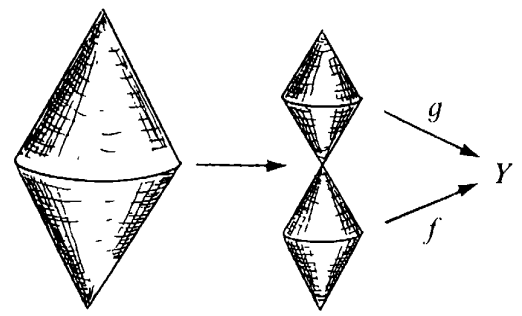
\includegraphics[width=0.6\textwidth]{Figures/TKISO0932.png}
      \caption{The product of two map classes
      $SX \to Y$.}
      \label{fig:TKISO0932-png}
  \end{figure}


  For a map $f \colon \left( SX, \left\{ A \right\}  \right) 
  \to \left( Y, \left\{ y_0 \right\}  \right) $, we denote its
  homotopy class in
  $\left[ SX; Y \right]_{*}$ by
  $\left[ f \right] $, and we define
  \[
  \left[ f \right] \left[ g \right] =
  \left[ f*g\right] 
  \] 
  Under this operation, the set
  $\left[ SX;Y \right]_*$ becomes a group.

  \begin{proposition}[]
      The reduced suspension gives
      $S S^{n-1}\cong S^{n}$.
  \end{proposition}

  Thus, we can define $S^{n}$ as the $n$-fold reduced
  suspension of $S^{0}$. As a special case,
  the set $\left[ S^{n};Y \right]_*$ then becomes
  a group for $n>0$. 

  \begin{definition}[$n$ th homotopy group]
      We define
      \[
      \pi_n \left( Y, y_0 \right) =
      \left[ S^{n}; Y \right]_*
      \] 
      with this operation.
  \end{definition}

  \subsection{Homotopy Groups using H-Spaces/Groups/Cogroups}

  From now on, unless otherwise indicated, we regard
  the $n$-sphere $S^{n}$ as having the cogroup
  structure as the reduced suspension
  $S^{n} = S S^{n-1} = S^{n-1} \wedge S^{1}$ - i.e.,
  the map $\gamma$ in the definition of an H-cogroup will
  be $\gamma \colon S^{n} \to S^{n} \vee S^{n}$ 
  given by
  \[
  \gamma(t,x) = 
  \begin{cases}
      \left( 2t,x \right)_{1},& t\le \frac{1}{2}\\
      \left( 2t-1, x \right)_2,& t\ge \frac{1}{2}.
  \end{cases}
  \] 
  The
  $0$-sphere $S^{0}$ is $\left\{ 0,1 \right\} $ 
  with base point $\left\{ 0 \right\} $.\\

  For a based space $X$ with base point $x_0$, we define
  the nth homotopy group
  \[
  \pi_n (X,x_0) = 
  \left[ S^{n},* ; X, x_0 \right] .
  \] 
  This is a group with the product defined by
  Theorem \ref{Thm:H-group-cogroup}.(2).

  \begin{theorem}[]\label{Theorem:Htpy-Groups-Abelian}
      If $X$ is an H-space then the multiplication
      in $\pi_n (X,x_0)$ is induced by
      the H-space multiplication and is abelian for
      $n\ge 1$.
  \end{theorem}

  \begin{proof}
      This follows directly from Theorem \ref{Thm:H-group-cogroup}.
  \end{proof}

  \begin{lemma}[]\label{Lemma:Suspension-Loop-Space}
      In the pointed category,
      $\left[ SX ; Y \right] \cong
      \left[ X ; \Omega Y \right]$ as groups.
  \end{lemma}
  
  \begin{proof}
      Recall the characteristic correspondence for
      the compact-open topology (Theorem \ref{Thm:Compact-Open-Top}):
      \[
      f\colon X \times S^{1} \to Y 
      \leftrightarrow f' \colon X \to Y^{S^{1}}
      \] 
      given by
      $f'(x) (t) = f(x,t)$.
      Recall that $SX = X \wedge S^{1}$, so
      a map
      $g \colon X \wedge S^{1} \to Y$ induces a map
      $f \colon X \times S^{1} \to Y$ by
      the composition 
      $X \times S^{1} \to X \wedge S^{1} \stackrel{g}{\to} Y$.
      Then $f$ is continuous if and only if
      the map $f' \colon X \to Y^{S^{1}}$ is continuous, where
      $f'(x)(*) = f(x,*) = *$, so
      $f'(*) = * \in Y^{S^{1}}$, the basepoint
      of $\Omega Y$.
      So the correspondence induces a bijective
      correspondence between pointed maps
      $SX \to Y$ and pointed maps $X \to \Omega Y$, and
      pointed homotopies correspond as well.\\
      It remains to show that the correspondence
      is a group homomorphism.
      Recall that $SX$ is an H-cogroup and
      $\Omega X$ is an H-group, so using
      Theorem \ref{Thm:H-group-cogroup}, we
      get that 
      for $f,g \colon SX \to Y$, the product in
      $\left[ SX;Y \right] $ is induced by
      \[
          \left( f*g \right) (x,t) = 
          \begin{cases}
              f(x,2t),& t\le \frac{1}{2}\\
              g\left( x,2t-1 \right),& t\ge \frac{1}{2},
          \end{cases}
      \] 
      which is equal to
      $\left( f*g \right)'(x)(t)$, 
      while the multiplication in
      $\left[ X ; \Omega Y \right] $ is given by
      $\left( f' \cdot g' \right) (x) = 
      f'(x) * g'(x)$ where $*$ is loop concatenation. 
      At time $t$, this is
      $f'(x) (2t)$ for $t\le \frac{1}{2}$ and
      $g'(x) (2t-1)$ for $t\ge \frac{1}{2}$. Thus
      $\left( f*g \right) ' = f' \cdot  g'$.
  \end{proof}


  All of the above immediately carries over to pointed
  pairs $(X,A)$ with a base point in $A$, so
  $\left[ SX, SA ; Y,B \right] $ is a group that
  is canonically isomorphic to
  $\left[ X,A; \Omega Y, \Omega B \right] $.

  Note in particular that
  $D^{n} \cong S D^{n-1}$ for all $n\ge 2$, so
  $D^{n} = D^{1} \wedge S^{n-1} \supset 
  S^{0} \wedge S^{n-1} = S^{n-1}$, so
  $\left( D^{n}, S^{n-1} \right) 
  = S^{n-1} \left( D^{1}, S^{0} \right) $, the
  $(n-1)$-fold reduced suspension. Hence
  we can define the relative homotopy group by
  \[
  \pi_n \left( Y,B,* \right) =
  \left[ D^{n}, S^{n-1}; Y ,B \right] 
  = \left[ S^{n-1}\left( D^{1}, S^{0} \right) ;
  Y,B\right] .
  \] 
  Note that this is defined on pointed spaces and pointed maps,
  so this set is really
  $\left[ D^{n},S^{n-1},s_0; Y,B, * \right] $.
  This becomes a group for $n\ge 2$. 

  Next note that we have a quotienting map
  \[
      I^{n} = \underbrace{D^{1}}_{=I} \times I \times \ldots \times I
      \to D^{1} \wedge S^{1} \wedge \ldots
      \wedge S^{1} =
      D^{n}.
  \] 
  Under this map, 
  $\partial I^{n}$ corresponds to
  $S^{n-1}$ and
  the base point corresponds to
  $J^{n-1} = \left( I \times \partial I^{n-1} \right) 
  \cup  \left( \left\{ 0 \right\} \times I^{n-1} \right) $.
  Thus under this quotienting map, we obtain a
  bijection
  \[
  \pi_n(Y,B,*) =
  \left[ D^{n}, S^{n-1},s_0; Y,B, * \right] 
  \cong \left[ I^{n}, \partial I^{n}, J^{n-1};
  Y,B,*\right].
  \] 

  \begin{corollary}
      $\pi_n(Y,*)$ is abelian for
      $n\ge 2$ and $\pi_n (Y,B,*)$ is abelian for
      $n\ge 3$. Moreover, the group structure is
      independent of the suspension coordinate used
      to define it.
  \end{corollary}

  \begin{proof}
      Recall from Lemma \ref{Lemma:Suspension-Loop-Space}, that
      $\left[ S^{n};Y \right] 
      = \left[ S^{1} \wedge \ldots \wedge S^{1};Y \right] 
      \cong \left[ S^{n-1} ; \Omega Y \right] $ as
      groups. Now
      the loop structure corresponds to the suspension in
      the last coordinate by definition, and
      by Theorem \ref{Thm:H-group-cogroup}, this
      is the same as the group 
      $\left[ S^{n};Y \right] $ with the suspension
      operation on any of the coordinates, since
      the choice of coordinate is arbitrary, this
      shows that
      the group structure on $\pi_n(Y,*) =
      \left[ S S^{n-1};Y \right]
      = \left[ S^{1} \wedge \ldots \wedge
      S^{1}; Y \right] $ is independent
      of the suspension coordinate used to define it.\\
      The product in $\left[ S^{n-1}; \Omega Y \right] $ is
      furthermore abelian for $n-1 \ge 1$ by
      Theorem \ref{Theorem:Htpy-Groups-Abelian} (using that
      $\Omega Y$ is an H-space), and
      the relative case is similar.
  \end{proof}

  \begin{corollary}
      \[
      \pi_n\left( Y,* \right) \cong
      \pi_{n-1}\left( \Omega Y, * \right) 
      \cong \ldots \cong
      \pi_1\left( \Omega^{n-1}Y,* \right) 
      \cong \pi_0 \left( \Omega^{n}Y ,* \right) 
      \] 
      and similarly in the relative case.
  \end{corollary}

  \begin{theorem}[]\label{Thm:Bredon-4.5}
      Let $A$ be a closed subspace of $X$ containing the
      base point $*$. Suppose that $F \colon X \times I \to X$ 
      is a deformation of $X$ contracting $A$ to
      $*$ ; i.e.,
      \begin{align*}
          F(A \times I) 
          &\subset A\\
          F(x,0) 
          &= x\\
          F\left( A \times \left\{ 1 \right\}  \right) 
          &= *\\
          F\left( \left\{ * \right\} \times I \right) 
          &= *
      \end{align*}
      then the quotient map $X \to X /A$ is a homotopy equivalence.
      Similarly for pairs $\left( X,X' \right) $ with
      $A \subset X'$.
  \end{theorem}

  \begin{proof}
      Let
      $\psi \colon X / A \to X$ be defined by the
      commutative diagram
      \begin{equation*}
      \begin{tikzcd}
          X \ar[d, "\varphi "] 
          \ar[dr, "F_{X \times \left\{ 1 \right\} } "]& \\
          X / A \ar[r, "\psi"] & X
      \end{tikzcd}
      \end{equation*}
      We claim that. Let $\varphi \colon X \to X / A$ be
      the quotienting map. We claim that
      $\psi \varphi \simeq \id_{X}$ and
      $\varphi \psi \simeq \id_{X / A}$.
      Since $F\left( A \times I \right) \subset A$, 
      $F$ induces a homotopy
      $F' \colon X / A \times I \to X / A$, where
      $F_{X / A \times \left\{ 1 \right\} }
      = \varphi \psi $, so
      since $F_{X / A \times \left\{ 0 \right\} }
      = \id_{X / A}$, we get the result.
  \end{proof}


  \newpage




  \subsubsection{A different way of defining
  $\pi_n \left( Y, y_0 \right) $}
  Note that reduced suspension supplies a parameter in
  $\left[ 0,1 \right] $ and the space
  $S^{n}$ as constructed is the quotient space of
  $I^{n}$ obtained by collapsing the boundary of the cube to a
  point.
  Pointed maps $S^{n}\to Y$ are in bijective correspondence
  with maps $I^{n}\to Y$ taking $\partial I^{n}$ to
  the base point of $Y$. This is a more traditional way
  of defining $\pi_n(Y)$. This becomes the group
  of homotopy classes of maps
  $\left( I^{n},\partial I^{n} \right) \to 
  \left( Y, \left\{ y_0 \right\}  \right) $ with the
  operation being
  \[
  f*g \left( t_1, \ldots, t_n \right) =
  \begin{cases}
      f\left( 2t_1, t_2, \ldots, t_n \right) ,& t_1 \in 
      \left[ 0,\frac{1}{2} \right] \\
      g\left( 2t_1-1, t_2, \ldots, t_n \right) ,& t_1 \in 
      \left[ \frac{1}{2},1 \right] 
  \end{cases}.
  \] 

  \begin{proposition}[]
      For $n\ge 2$, $\pi_n\left( X, x_0 \right)$ is abelian.
  \end{proposition}

  \begin{proof}
      Consider the homotopy in Figure \ref{fig:JIDWOOL0290L-png}.
      We begin by shrinking the domains of $f$ and $g$ to smaller
      subcubes of $I^{n}$, where the region outside is
      mapped to the basepoint. This allows us to move the boxes
      around in a continuous manner. The rest is clear.
      \begin{figure}[htpb]
          \centering
          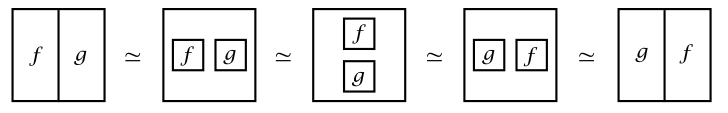
\includegraphics[width=0.8\textwidth]{Figures/JIDWOOL0290L.png}
          \caption{The homotopy in question}
          \label{fig:JIDWOOL0290L-png}
      \end{figure}
  \end{proof}

  Next, we want to show that following:
  \begin{proposition}[]\label{Prop:SwjiaKKDNW1102}
      If $X$ is path-connected, then
      $\pi_n\left( X, x_0 \right) \cong
      \pi_n (X, x_1)$ for any two $x_0,x_1 \in X$.
  \end{proposition}

  For this, we introduce an action of
  $\pi_1$ on $\pi_n$.

  \begin{definition}[The action of $\pi_1$ on $\pi_n$]
      Given a path
      $\gamma \colon I \to X$ from
      $x_0$ to $x_1$, we associate to a map
      $f \colon \left( I^{n}, \partial I^{n} \right) \to 
      \left( X, x_1 \right) $ the map
      $\gamma f \colon \left( I^{n}, \partial I^{n} \right) 
      \to \left( X,x_0 \right) $ by shrinking the domain
      of $f$ to a smaller concentric cube in $I^{n}$, then
      inserting the path $\gamma$ on each radial segment
      in the shell between this smaller cube and $\partial
      I^{n}$.
      See Figure \ref{fig:JDWIXHHX011SJ-png}

      \begin{figure}[htpb]
          \centering
          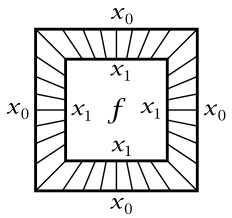
\includegraphics[width=0.25\textwidth]{Figures/JDWIXHHX011SJ.png}
          \caption{Depiction of $\gamma f$.}
          \label{fig:JDWIXHHX011SJ-png}
      \end{figure}

  \begin{note}
      We have the following properties
      \begin{enumerate}
          \item $\gamma \left( f+ g \right) 
              \simeq \gamma f + \gamma g$.
          \item $\left( \gamma \eta \right) f \simeq
              \gamma \left( \eta f \right) $.
          \item $\id f \simeq f$, where
              $\id$ denotes the constant path.
      \end{enumerate}

      To see $(1)$, first deform $f$ and $g$ to be
      constant on the right and left halves of
      $I^{n}$, respectively, producing maps
      which we may call $f+0$ and $0+g$, then we 
      can excise a progressively wider symmetric middle slab
      of $\gamma (f+0) + \gamma(0+g)$ (which can be
      seen on the left in Figure \ref{fig:WIWIWSSK11-png})
      until it becomes $\gamma \left( f+g \right) $ (shown on the
      right).

      \begin{figure}[htpb]
          \centering
          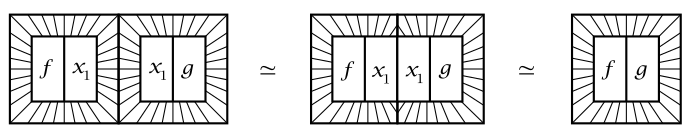
\includegraphics[width=0.8\textwidth]{Figures/WIWIWSSK11.png}
          \caption{}
          \label{fig:WIWIWSSK11-png}
      \end{figure}
  \end{note}

  Now if $\beta_{\gamma} \colon \pi_n(X,x_1) \to 
  \pi_n(X, x_0)$ is the change-of-basepoint transformation,
   $\beta_{\gamma}\left[ f \right] =
   \left[ \gamma f \right] $, then
   the above note shows that $\beta_\gamma$ is a group isomorphism.
   This proves Proposition \ref{Prop:SwjiaKKDNW1102}. 
   If we restrict attention to loops
   $\gamma$ at $x_0$, then since $\beta_{\gamma \eta}=
   \beta_{\gamma} \beta_{\eta}$, the map
   $\left[ \gamma \right] \mapsto \beta_{\gamma}$ 
   defines a homomorphism from
   $\pi_1\left( X, x_0 \right) $ to
   $\Aut \left( \pi_n \left( X,x_0 \right)  \right) $ 
   called the \textit{action of $\pi_1$ on $\pi_n$ }.
  \end{definition}

  \begin{note}
  For $n>1$, this action makes
  $\pi_n(X,x_0)$ into a module over the group ring
  $\mathbb{Z}\left[ \pi_1 \left( X,x_0 \right)  \right] $.
  \end{note}  

  \begin{definition}[Simple/abelian spaces]
      A space with trivial $\pi_1$ action on $\pi_n$ is called
      '$n$-simple', and 'simple' means
      ' $n$-simple for all $n$ '. We call
      a space \textit{abelian} if it has
      trivial action of $\pi_1$ on all homotopy groups
      $\pi_n$.
  \end{definition}

  \begin{proposition}[$\pi_n$ is a functor]
      A map $\varphi  \colon \left( X, x_0 \right) \to 
      \left( Y, y_0 \right) $ induces a map
      $\varphi_* \colon \pi_n \left( X, x_0 \right) \to 
      \pi_n \left( Y, y_0 \right) $ defined by
      $\varphi_* \left[ f \right] = \left[ \varphi  f \right] $.
      It is immediate from the definitions that
      $\varphi_*$ is well-defined and a homomorphism
      for $n\ge 1$. The functorial properties are also clear.
  \end{proposition}

  \begin{corollary}
      Homotopy equivalent spaces have isomorphic
      homotopy groups.
  \end{corollary}

  \begin{proposition}[]
      A covering space projection
      $p \colon \left( \tilde{X}, \tilde{x}_0 \right) \to 
      \left( X, x_0 \right) $ induces isomorphisms
      $p_* \colon \pi_n \left( \tilde{X}, \tilde{x}_0 \right) 
      \to \pi_n \left( X, x_0 \right) $ for all
      $n \ge 2$.
  \end{proposition}

  \begin{proof}
      Since 
      $S^{n}$ is path-connected and locally path-connected,
      and simply connected for $n\ge 2$, we find that
      any map
      $\left( S^{n},s_0 \right) 
      \to \left( X, x_0 \right) $ lifts to a 
      map $\left( S^{n},s_0 \right) \to 
      \left( \tilde{X},\tilde{x}_0 \right) $ when
      $n\ge 2$. This gives surjectivity of
      $p_*$.
      For injectivity, suppose
      $p_* \left[ f \right] = \left[ 0 \right] $ where
      $f \colon \left( S^{n}, s_0 \right) \to 
      \left( \tilde{X},\tilde{x}_0 \right) $.
      Let $c_{\tilde{x}_0}$ be the constant map at
      $\tilde{x}_0$. Then
      $p_* \left[ \tilde{x}_0 \right] =
      \left[ 0 \right] $, so by uniqueness of the
      lifting theorem, 
      $\left[ f \right] = \left[ c_{\tilde{x}_0} \right] =
      \left[ 0 \right] $.
  \end{proof}

  \begin{definition}[Aspherical]
      Spaces with $\pi_n = 0$ for all
      $n\ge 2$ are called \textit{aspherical}.
  \end{definition}

  \begin{corollary}
      $S^{1}, T^{n}$ and $K$ are aspherical since
      they have contractible covering spaces.
  \end{corollary}


  \begin{proposition}[]
      \[
      \pi_n \left( \prod_{\alpha} X_{\alpha} \right) 
      \cong \prod_{\alpha} \pi_n \left( X_{\alpha} \right) 
      \] 
  \end{proposition}

  Next we define relative homotopy groups.

  \begin{definition}[Relative homotopy groups]
      Regard $I^{n-1}$ as a face of $I^{n}$ with the last
      coordinate $s_n = 0$ and let
      $J^{n-1}$ be the closure of
      $\partial I^{n}- I^{n-1}$. Then
      we define 
      \[
      \pi_n \left( X, A, x_0 \right) 
      := \left[ I^{n},\partial I^{n}, J^{n-1};
      X , A , x_0\right] 
      \] 
      We shall leave $\pi_0 \left( X, A, x_0 \right) $ undefined
      for now.
  \end{definition}

  We can define a sum operation on $\pi_n \left( X, A, x_0 \right) $ 
  in the same way as for $\pi_n \left( X, x_0 \right) $, except
  now the coordinate $s_n$ now must remain free, so
  we must use one of the other coordinates. Thus
  we must have at least one other coordinate to define
  the same operation. So $\pi_n \left( X, A, x_0 \right) $ is
  a group for $n\ge 2$, and it is abelian for
  $n\ge 3$. For $n=1$, we have
  $I^{1} = \left[ 0,1 \right] , I^{0} = \left\{ 0 \right\} $ 
  and $J^{0} = \left\{ 1 \right\} $, so
  $\pi_1 \left( X, A, x_0 \right) 
  = \left[ I, \left\{ 0 \right\} , \left\{ 1 \right\} ;
  X, A, x_0 \right] $ is the set of homotopy classes of paths in
  $X$ from a varying point in $A$ to the fixed basepoint
  $x_0 \in A$. In general, this is not a group in any
  natural way. \\
  \linebreak
  Now, we saw before that
  $\pi_n \left( X, x_0 \right) $ can be regarded as
  homotopy classes of maps $\left( S^{n}, x_0 \right) \to 
  \left( X, x_0 \right) $. Similarly, collapsing
  $J^{n-1}$ to a point, converts
  $\left( I^{n} , \partial I^{n}, J^{n-1} \right) $ 
  to $\left( D^{n}, S^{n-1}, s_0 \right) $.
  In this case, addition is done by
  the map $c \colon D^{n} \to D^{n} \vee D^{n}$ collapsing
  $D^{n-1} \subset D^{n}$ to a point.\\
  \linebreak
  \begin{theorem}[Compression criterion]\label{Thm:Compression}
      A map $f \colon \left( D^{n}, S^{n-1}, s_0 \right) 
      \to \left( X, A, x_0 \right) $ represents zero
      in $\pi_n \left( X, A, x_0 \right) $ if and only if
      it is homotopic $\rel S^{n-1}$ to a map with image
      contained in $A$.
  \end{theorem}
  
  \begin{proof}
      Suppose we have a homotopy
      $\rel S^{n-1}$ from $f$ to a map
      $g$, so
      $\left[ f \right] = \left[ g \right] $ in
      $\pi_n \left( X, A, x_0 \right) $. 
      Viewing $g$ as a map
      $\left( D^{n}, S^{n-1}, s_0 \right) 
      \to \left( X, A, x_0 \right) $ whose
      image is contained in $A$, we
      can construct the homotopy
      $H \colon D^{n} \times I \to X$ by
      $H(x,t) = g\left( (1-t) x + s_0 t \right) $ 
      which is a homotopy from $g$ to the
      constant map at $x_0$, hence
      $\left[ g \right]  = 0$ in $\pi_n (X, A, x_0)$.\\
      Conversely, if $\left[ f \right] = 0$ via
      a homotopy $F \colon D^{n} \times I \to X$ such that
      $F(x,0) = f(x)$ and
      $F(x,1) = x_0$ for all $x \in D^{n}$ and
      $F(x,t) \in A$ for all
      $x$ with $\left| x \right| = 1$ as well
      as $F(s_0,t) = x_0$ for all $t$. We can
      construct a homotopy
      using $F$ by restricting $F$ to a family of
      $n$-disks in $D^{n} \times I$ starting with
      $D^{n}\times \left\{ 0 \right\} $ and ending
      with the disk $D^{n} \times \left\{ 1 \right\} 
      \cup S^{n-1} \times I$, and where all the disks
      throughout the family have the same boundary.
      See Figure \ref{fig:DJIMMXKXO0O-jpeg} for a depiction
      of this homotopy.

      \begin{figure}[htpb]
          \centering
          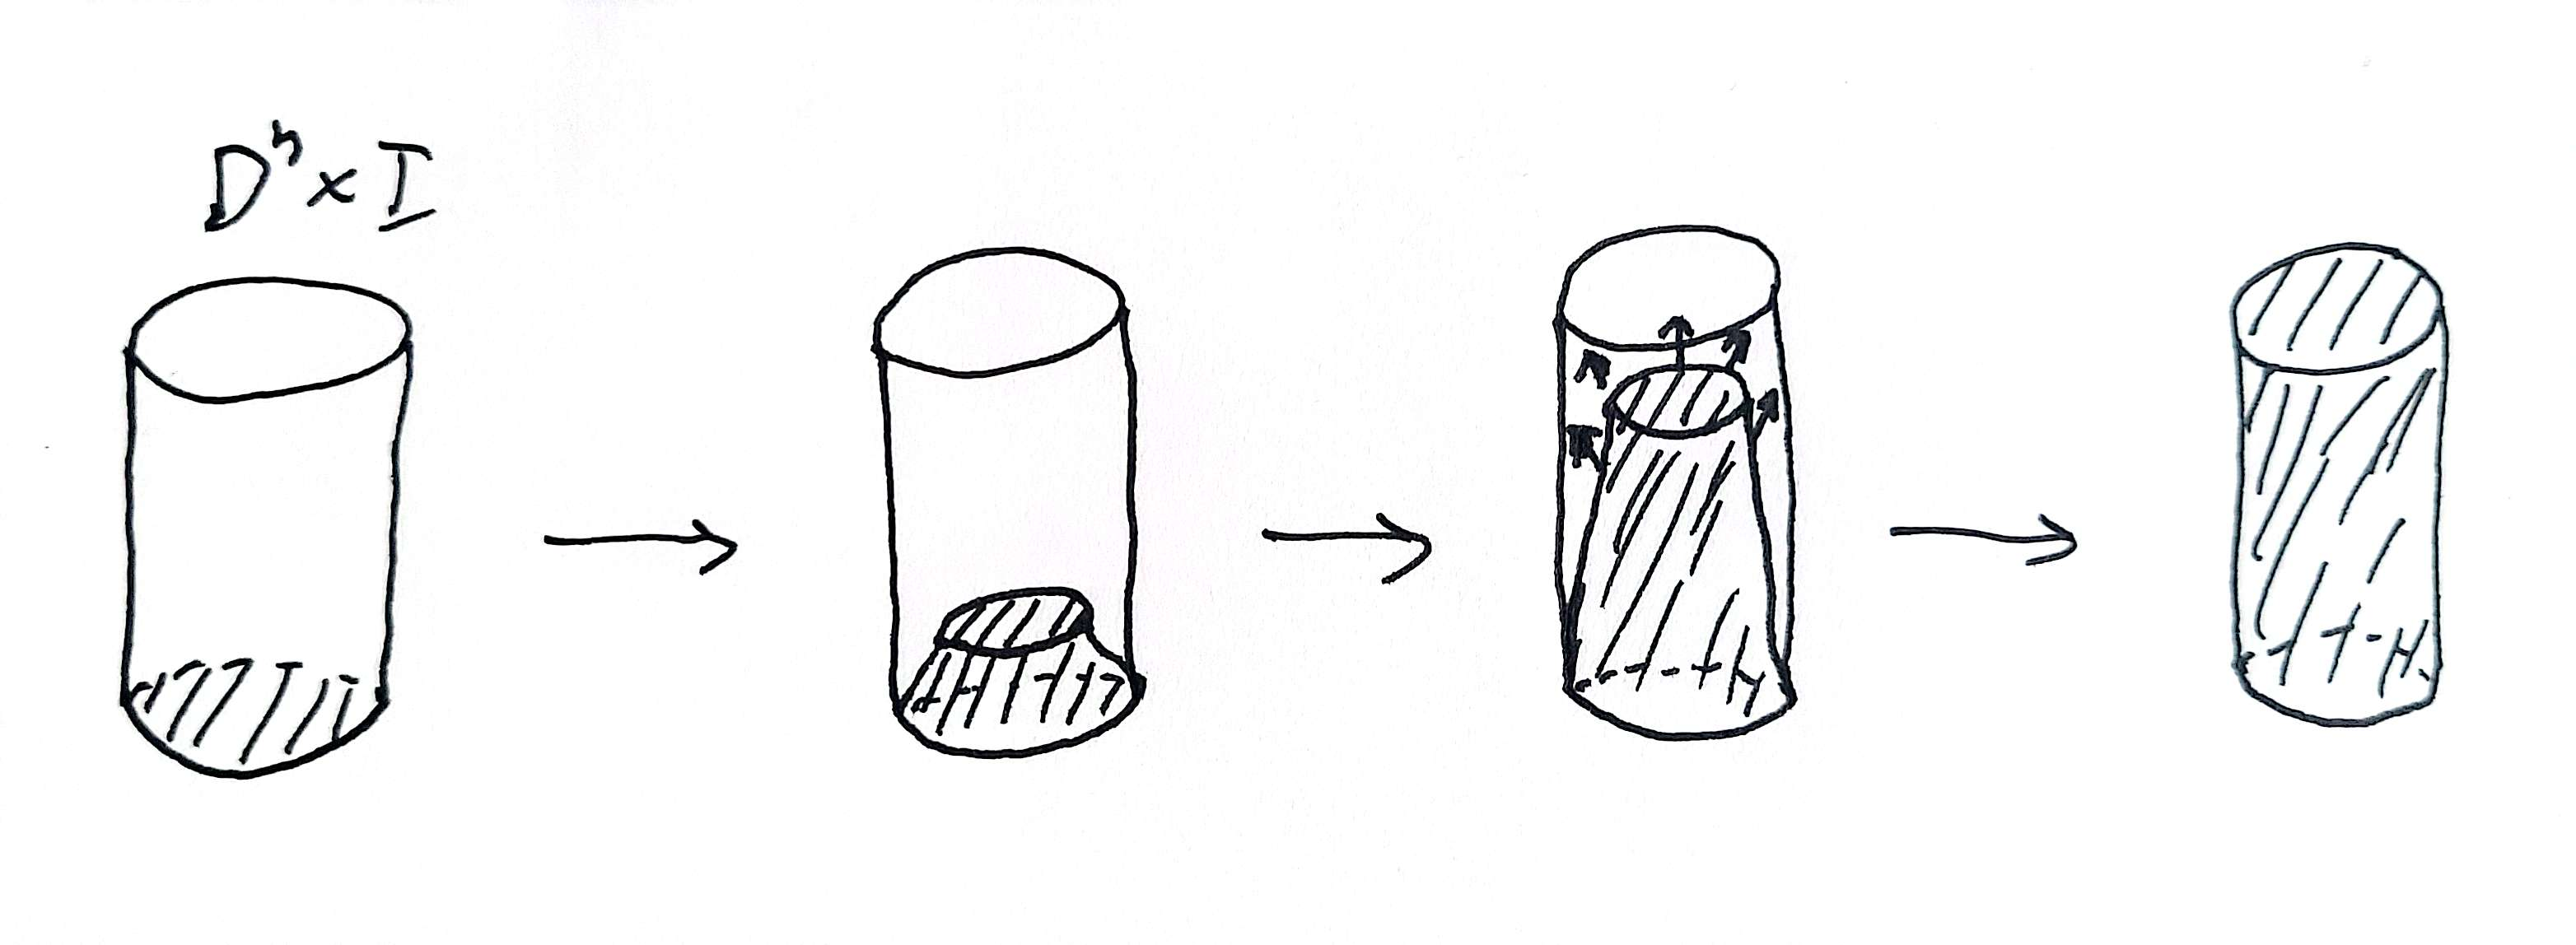
\includegraphics[width=0.8\textwidth]{Figures/DJIMMXKXO0O.jpeg}
          \caption{}
          \label{fig:DJIMMXKXO0O-jpeg}
      \end{figure}
      This completes the proof.
  \end{proof}

  Next, some things that carry over:
  a map $\varphi \colon \left( X, A, x_0 \right) 
  \to \left( Y, B, y_0 \right) $ induces maps
  $\varphi_* \colon \pi_n \left( X, A, x_0 \right) 
  \to \pi_n \left( Y, B, y_0 \right) $ which are
  homomorphisms when $n\ge 2$ and have properties analogous
  to those in the absolute case: 
  $\left( \varphi \psi  \right)_* = 
  \varphi_* \psi_*, (\id_{(X,A,x_0)})_{*} = \id_{\pi_n (X, A, x_0)}$,
  and if  $\varphi \simeq \psi $ through maps
  $\left( X,A,x_0 \right) \to \left( Y,B,y_0 \right) $,
  then $\varphi_* = \psi_*$. 

  \subsubsection{LES of relative homotopy groups}
  Probably the most useful feature of relative homotopy
  groups $\pi_n (X,A,x_0)$ is that they 
  fit into a long exact sequence
  \[
  \ldots \to \pi_n (A,x_0)
  \stackrel{i_*}{\to} \pi_n(X,x_0)
  \stackrel{j_*}{\to} \pi_n (X,A,x_0)
  \stackrel{\partial}{\to} \pi_{n-1}(A,x_0) \to 
  \ldots \to \pi_0 (X,x_0).
  \] 
  Here $i$ and $j$ are the inclusions
  $\left( A, x_0 \right) \hookrightarrow
  (X,x_0)$ and
  $\left( X, x_0, x_0 \right) \hookrightarrow
  \left( X,A,x_0 \right) $. The map
  $\partial$ comes from restricting maps
  $\left( I^{n},\partial I^{n}, J^{n-1} \right) \to 
  \left( X,A,x_0 \right) $ to
  $I^{n-1}$ (the face of $I^{n}$ with the last
  coordinate $s_n = 0$ ),
  or equivalently, by restricting maps
  $\left( D^{n},S^{n-1},s_0 \right) \to 
  \left( X,A,x_0 \right) $ to $S^{n-1}$. The map $\partial$,
  called the \textit{boundary map}, is a homomorphism
  when $n>1$. In fact, we can show the following theorem

  \begin{theorem}[LES of relative homotopy groups]
      Given 
      $x_0 \in B \subset A \subset X$,
      the sequence of relative homotopy groups
  \[
      \ldots \to 
      \pi_n \left( A,B, x_0 \right) 
      \stackrel{i_*}{\to} 
      \pi_n \left( X, B, x_0 \right) 
      \stackrel{j_*}{\to} 
      \pi_n (X, A, x_0)
      \stackrel{\partial}{\to} 
      \pi_{n-1} \left( A,B, x_0 \right) 
      \to \ldots \to 
      \pi_1 (X,A,x_0)
  \] 
  is exact and natural.
  In the case when $B = \left\{ x_0 \right\} $, we have that
  the LES
  \[
  \ldots \to \pi_n (A,x_0)
  \stackrel{i_*}{\to} \pi_n(X,x_0)
  \stackrel{j_*}{\to} \pi_n (X,A,x_0)
  \stackrel{\partial}{\to} \pi_{n-1}(A,x_0) \to 
  \ldots \to \pi_0 (X,x_0).
  \] 
  is exact and natural.
  \end{theorem}

  \begin{proof}
      \textit{Exactness at $\pi_n
      \left( X,B,x_0 \right) $ :} the composition
      $j_* i_*$ is zero because any
      map $\left( I^{n}, \partial I^{n},
      J^{n-1}\right) \to \left( A,B,x_0 \right) $ 
      is zero in $\pi_n \left( X, A, x_0 \right) $ by the
      compression criterion (Theorem \ref{Thm:Compression}).
      To see that $\ker j_* \subset 
      \im i_*$, let
      $f \colon \left( I^{n}, \partial I^{n},
      J^{n-1}\right) \to \left( X, B, x_0 \right) $ 
      represent zero in $\pi_n \left( X, A, x_0 \right) $.
      Using the compression criterion again, we
      then get that $f$ is homotopic $\rel \partial I^{n}$ 
      to a map with image in $A$, hence the class
      $\left[ f \right] \in \pi_n \left( X, B, x_0 \right) $ 
      is indeed in the image of $i_*$. We conclude that
      $\ker j_* = \im i_*$, obtaining exactness
      at $\pi_n \left( X,B, x_0 \right) $.\\
      \textit{Exactness at $\pi_n (X,A,x_0)$:} 
      for a map  $\left[ f \right] 
      \in \im j_*$, we have that
      $j_*$ maps $\partial I^{n}$ into $B$, hence
      in particular $I^{n-1} \subset \partial I^{n}$ into
      $B$, so $\partial j_* \left[ f \right] $ 
      represents a homotopy class
      in $\pi_{n-1}\left( A,B,x_0 \right) $ with
      image in $B$, but then by the compression criterion,
      $\partial j_* \left[ f \right] = 0$ in
      $\pi_{n-1} \left( A,B,x_0 \right) $, so
      $\im j_* \subset \ker \partial $.
      Conversely, suppose
      $\partial \left[ f \right] = 0$. By the compression
      criterion, representatives of $\partial \left[ f \right] $
      are homotopic $\rel \partial I^{n-1}$ to a map
      with image in $B$. In particular,
      $f|_{I^{n-1}}$ is homotopic to a map with
      image in $B$ via a homotopy $F \colon
      I^{n-1} \times I \to A \rel \partial I^{n-1}$.
      We can tack $F$ onto $f$ to get a new map
      $\left( I^{n}, \partial I^{n},
      J^{n-1}\right) \to 
      \left( X, B, x_0 \right) $ which, as
      a map
      $\left( I^{n}, \partial I^{n}, J^{n-1} \right) \to 
      \left( X, A, x_0 \right) $ is homotopic to
      $f$ by the homotopy that tacks on increasingly longer
      initial segments of $F$. See Figure
      \ref{fig:IDIWKAKX-png}. Hence
      $\left[ f \right] \in \im j_*$.

      \begin{figure}[htpb]
          \centering
          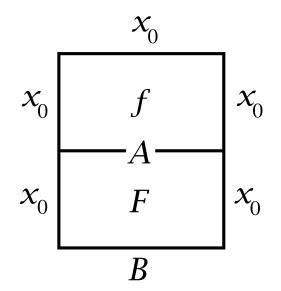
\includegraphics[width=0.2\textwidth]{Figures/IDIWKAKX.png}
          \caption{}
          \label{fig:IDIWKAKX-png}
      \end{figure}

      \textit{Exactness at $\pi_n (A,B,x_0)$ :} 
      First, $i_* \partial$ is zero since
      the restriction of a map
      $f \colon \left( I^{n+1}, \partial I^{n+1},
      J^{n}\right) \to \left( X,A,x_0 \right) $ 
      to $I^{n}$ is homotopic $\rel \partial I^{n}$ to a 
      constant map via $f$ itself (a similar picture
      to Figure \ref{fig:DJIMMXKXO0O-jpeg} works).\\
      Conversely, if $B$ is a point, then
      a nullhomotopy $f_t \colon
      \left( I^{n}, \partial I^{n} \right) 
      \to \left( X, x_0 \right) $ of
      $f_0 \colon \left( I^{n},\partial I^{n} \right) 
      \to \left( A,x_0 \right) $ gives a map
      $F \colon \left( I^{n+1},\partial I^{n+1},J^{n} \right) 
      \to \left( X,A,x_0 \right) $ with
      $\partial \left( \left[ F \right]  \right) 
      = \left[ f_0 \right] $. So in this case, the proof is
      finished.
      For a general $B$, let
      $F$ be a nullhomotopy of
      $f \colon \left( I^{n},\partial I^{n},J^{n-1} \right) 
      \to \left( A,B,x_0 \right) $ through maps
      $\left( I^{n}, \partial I^{n}, J^{n-1} \right) 
      \to \left( X,B,x_0 \right) $ and
      let $g$ be the restriction of
      $F$ to $I^{n-1}$ in $I^{n-1} \times I = I^{n}$ (see
      the first of the pictures in
      Figure \ref{fig:USIIOOQ-png}).
      Next reparametrize the $n$ th and
      $(n+1)$ st coordinates as in the
      second picture. Then 
       we find that $f$ with $g$ tacked on
       is in the image of $\partial$. But
       as before, tacking $g$ onto $f$ gives the
       same element of $\pi_n (A,B,x_0)$

      \begin{figure}[htpb]
          \centering
          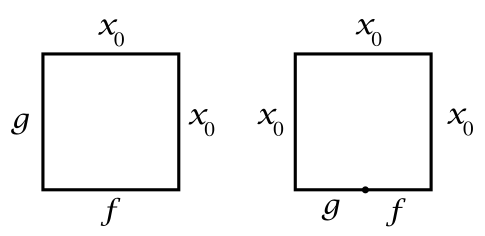
\includegraphics[width=0.4\textwidth]{Figures/USIIOOQ.png}
          \caption{}
          \label{fig:USIIOOQ-png}
      \end{figure}
  \end{proof}

  
\begin{corollary}
    Consider the inclusion
    $\iota \colon X = X \times \left\{ 0 \right\} 
    \hookrightarrow CX$.
    Then
    $\pi_n \left( CX, X, x_0 \right) 
    \cong \pi_{n-1}\left( X, x_0 \right) $ for all
    $n\ge 1$. Taking
    $n=2$, we can thus realize an group $G$, abelian
    or not, as a relative $\pi_2$ by
    choosing $X$ to have $\pi_1 (X) \cong G$.
\end{corollary}

There are also change-of-basepoint isomorphisms
$\beta_{\gamma}$ for relative homotopy groups.
One takes a path  $\gamma$ in $A \subset X$ from
$x_0$ to $x_1$ which induces
$\beta_{\gamma} \colon \pi_n (X,A,x_1) \to 
\pi_n (X,A,x_0)$ by setting
$\beta_{\gamma} \left( \left[ f \right]  \right) 
= \left[ \gamma f \right] $, where
$\gamma f$ is depicted in 
Figure \ref{fig:DIWIOA-png}.

\begin{figure}[htpb]
    \centering
    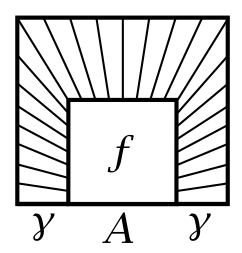
\includegraphics[width=0.2\textwidth]{Figures/DIWIOA.png}
    \caption{}
    \label{fig:DIWIOA-png}
\end{figure}

Restricting to loops at the
basepoint, the association $\gamma \mapsto 
\beta_{\gamma}$ defines an action
of $\pi_1 \left( A, x_0 \right) $ on
$\pi_n \left( X, A, x_0 \right) $ analogous to the
action of $\pi_1 \left( X, x_0 \right) $ on
$\pi_n (X,x_0)$.






%\subsection{Problem Set 1}

\subsubsection{Exercises}


\begin{exercise}[The action of the fundamental gorup, part
    2]
    Let $X$ be a path-connected, semi-locally simply-connected
    space with basepoint $x$ and $p \colon \tilde{X}\to X$ its
    universal cover. Show that for $n\ge 2$ and
     $\tilde{x} \in X$ with $p (\tilde{x}) = x$, the isomorphism
     $p_* = \pi_n (p) \colon \pi_n \left( \tilde{X}, \tilde{x} \right) 
     \cong \pi_n(X, x)$ allows us to identify the
     action of $\pi_1 \left( X, x \right) $ on $\pi_n (X, x)$ with
     the action of $\pi_1 \left( X, x \right) $ on
     $\pi_n \left( \tilde{X}, \tilde{x} \right) $ induced by
     the group of deck transformations, i.e., the natural action
     of $\pi_1 (X, x)$ on $\tilde{X}$. In particular, make the
     statement precise.
\end{exercise}

\begin{proof}
    We want to show that for $\left[ \gamma \right] 
    \in \pi_1(X, x)$ and
    $\left[ f \right] \in \pi_n \left( X, x \right) $,
    if $\tilde{g}$ is the lift for $\gamma$ starting at
    $\tilde{x}_0$, and
    $\tilde{f} \colon \left( S^{n}, s_0 \right) 
    \to \left( \tilde{X}, \tilde{x}_0 \right) $ is the
    lift of $f$, then
    $p_* \left( \tilde{\gamma} \tilde{f} \right) 
    = \gamma f$. But this follows directly from how
    $\tilde{\gamma} \tilde{f}$ and 
    $\gamma f$ we constructed. Namely, applying
    $p$ to the square used in the definition, we see that we
    obtain $\gamma f$ from $\tilde{\gamma} \tilde{f}$ since
    $p \circ \tilde{\gamma} = \gamma$ and
    $p \circ \tilde{f} = f$.

\end{proof}


\begin{exercise}[]
    Let $X$ and $Y$ be pointed spaces and $n \ge 2$. Show that the
    inclusion $X \vee Y \hookrightarrow X \times Y$ induces
    a surjection $\pi_n \left( X \vee Y \right) 
    \to \pi_n \left( X \times Y \right) $ for all $n$. Furthermore,
    this exhibits $\pi_n \left( X \times Y \right) $ as
    a retract of $\pi_n \left( X \vee Y \right) $ for all $n$.
    (Is this also true for $n=1$?)
\end{exercise}

\begin{proof}
    a
\end{proof}






\subsubsection{Problems}

\begin{problem}[]\label{pset1-degree}
        Fix an isomorphism $H_n\left( S^{n} \right) \cong \mathbb{Z}$.
        We define the degree $\deg f$ of a map
        $f \colon S^{n} \to S^{n}$ to be the integer such that
        $f_* \colon H_n(S^{n}) \to H_n(S^{n})$ sends $1$ to
        $\deg f \in \mathbb{Z}$.
        \begin{enumerate}
            \item Show that taking the degree of a map
                $S^{n} \to S^{n}$ induces a well-defined
                map
                \[
                \deg \colon \pi_n(S^{n}) \to \mathbb{Z}
                \] 
            \item Show that $\deg $ is a group homomorphism.
            \item Show that the map $\deg$ is surjective.
            \item Suppose that $n\ge 2$. Show that
                $\pi_n\left( S^{n} \right) \cong
                \mathbb{Z} \times A$ for some abelian group $A$.
        \end{enumerate}
    \end{problem}

        \begin{proof}


        \begin{enumerate}
            \item Let
                $ \left[ f \right] 
                \in \pi_n \left( S^{n} \right) $ and
                suppose $f, f'$ are two representatives of
                this class. Then
                $f$ and $f'$ are homotopic by definition,
                so $f_* = \left( f' \right)_* \colon
                \mathbb{Z} = H_n\left( S^{n} \right) \to 
                H_n\left( S^{n} \right) = \mathbb{Z} $ are equal.
                In particular,
                $\deg f = f_*(1) = \left( f' \right)_* (1)
                = \deg f'$. So the map is well-defined.
            \item To show that degree is a group homomorphism,
                we must show that
                $\deg \left( f+g \right) = 
                \deg f + \deg g$.

                For this, we will show a couple of results.

                \begin{proposition}[]
                    Let $X = S_1^{n} \vee \ldots \vee
                    S_k^{n}$ for $n > 0$. Then
                    the homomorphism 
                    $H_n\left( S_1^{n} \right) \oplus \ldots
                    \oplus H_n\left( S_k^{n} \right) 
                    \to H_n(X)$ induced by the inclusion maps
                    is an isomorphism whose inverse
                    is induced by the projections
                    $X \to S_i^{n}$.
                \end{proposition}
                
                To prove this proposition, we must show the following
                lemma.

                \begin{lemma}[]
                    Let $X$ be a Hausdorff space and let
                    $x_0 \in X$ be a point having a closed
                    neighborhood $N$ in $X$ of which
                    $\left\{ x_0 \right\} $ is a strong deformation
                    retract. Let $Y$ be a Hausdorff space and
                    let $y_0 \in Y$. Define
                    $X \vee Y = X \times \left\{ y_0 \right\} 
                    \cup \left\{ x_0 \right\} \times Y$.
                    Then the inclusion maps induce
                    isomorphisms 
                    $\tilde{H}_i(X) \oplus \tilde{H}_i(Y)
                    \cong \tilde{H}_i\left( X \vee Y \right) $
                    whose inverse is induced by the projections
                    of $X \vee Y$ to $X$ and $Y$.
                \end{lemma}
                
                \begin{proof}[Proof of lemma]
                    Consider $A = X$ and
                    $U = X - N$ which is open, and
                    $\overline{U} \subset A$. Then by
                    excision,
                    $H_* \left( X \vee Y, X \right) 
                    \cong H_*\left( N \cup Y, N \right) 
                    \cong \tilde{H}_*\left( Y \right) $

                    Consider the LES of the triple
                    $\left( X \vee Y,
                    \left\{ x_0 \right\} \times Y,
                \left\{ x_0 \right\} \times 
            \left\{ y_0 \right\} \right) $. We obtain
            \[
            \ldots \to 
            H_p\left( \left\{ x_0 \right\} \times Y,
            \left( x_0,y_0 \right) \right)
            \stackrel{i_*}{\to}
            H_p\left( X \vee Y, \left( x_0,y_0 \right)  \right) 
            \stackrel{j_*}{\to} H_p\left( X \vee Y,
            \left\{ x_0 \right\} \times Y \right) \to \ldots
            \] 
            Since $\pi_Y \circ i = \id_{
            \left\{ x_0 \right\} \times Y} $, 
            $i_*$ is injective.

            Furthermore, we have
            \[
            H_p\left( X \vee Y, 
            \left( x_0, y_0 \right) \right) 
            \stackrel{\left( \pi_X \right)_* }{\to } 
            H_p \left( \left\{ x_0 \right\} \times Y,
            \left( x_0, y_0 \right) \right) 
            \cong H_p\left( X \vee Y , 
            \left\{ x_0 \right\} \times Y \right) 
            \] 
            so $j_* = \left( \pi_X \right)_*$ under these
            identifications, so, in particular, 
            $j_*$ is surjective. Therefore, our exact sequence
            is a SES:
            \[
            0 \to  H_p\left( Y, pt \right)
            \stackrel{i_*}{\to }
            H_p \left( X \vee Y, pt \right) 
            \stackrel{j_*}{\to }
            \underbrace{H_p \left( X \vee Y, Y \right)}_{
            \cong H_p\left( X, pt \right) } \to 0
            \] 
            It remains to show that this SES is split, but
            since
            $\pi_X \circ \iota_{X} = 
            \id_{\left\{ x_0 \right\} \times X}$,
            we have that $\iota_{X*}$ provides a section.

        \end{proof}

        \begin{proof}[Proof of proposition]
            This follows by induction on the lemma.
        \end{proof}

        Next, suppose that $E_1, \ldots, E_k$ are
        disjoint open subsets of $S^{n}$, each homeomorphic to
        $\mathbb{R}^{n}$ for $n>0$.
        Let $f \colon S^{n} \to Y$ be a map which takes
        $S^{n} - \bigcup E_i $ to $y_0$. Then
        $f$ factors through the quotient space
        $S^{n} / \left( S^{n} - \bigcup E_i  \right) 
        \cong S_1^{n} \vee \ldots \vee S_k^{n}$ where
        $S_i^{n} = S^{n} / \left( S^{n} - E_i \right) $:
        \[
            f \colon S^{n} \stackrel{g}{\to }
            S_1^{n} \vee \ldots \vee S_k^{n}
            \stackrel{h}{\to } Y
        \] 
        Let $\iota_{j} \colon S_j^{n} 
        \hookrightarrow S_1^{n} \vee \ldots \vee
        S_k^{n}$ be the $j$ th inclusion and let
        $p_j \colon S_1^{n} \vee \ldots \vee
        S_k^{n} \to S_j^{n}$ be the $j$ th projection.
        Then by the proposition,
        $\sum_j \iota_{j*} p_{j*} = \id_* \colon
        H_n \left( S_1^{n} \vee \ldots \vee S_k^{n} \right) 
        \to H_n \left( S_1^{n} \vee \ldots \vee
        S_k^{n}\right) $. Let
        $g_j = p_j \circ g \colon S^{n} \to S_j^{n}$ and
        $h_j = h \circ \iota_j \colon
        S_j^{n} \to Y$ and let
        $f_j = h_j \circ g_j \colon  S^{n} \to Y$.
        That is, $f_j$ is the map which is $f$ on
        $E_j$ and maps the complement of $E_j$ to the basepoint
        $y_0$.

        \begin{theorem}[]\label{Thm:Degree-of-sum-of-maps}
            In the above situation, $f_*
            = \sum_{j=1}^{k} f_{j*} \colon
            H_n\left( S^{n} \right) \to H_n(Y)$.
        \end{theorem}

        \begin{proof}[Proof of theorem]
            We have
            $f_* = 
            h_* \circ g_* = 
            \sum_j h_* i_{j*} p_{j*} g_*
            = \sum_j h_{j*} g_{j*}
            = \sum_j f_{j*}$.
        \end{proof}

        Now we get back to showing that
        $\deg \left( f+g \right) = \deg f + \deg g$.

        Note that by way of defining
        $f+g$, this essentially maps $I^{n}$ by
        $f$ on the left half and $g$ on the right half with
        the boundary mapping to the base point $x_0$.
        In particular, this factors through the
        quotient $I^{n} \to I^{n} / \partial I^{n} 
        \cong S^{n}$, where now the two halves can be interpreted
        as, say, the upper and lower hemispheres. In particular,
        the equator is by assumption also mapped to
        $x_0$, so we can quotient further by
        $S^{n} \to S^{n} \vee S^{n}$ by "pinching" the equator
        to a point. This is essentially what the proposition
        above describes. In particular, $f+g$ can be covered
        by the two open hemispheres and maps the equator
        to $x_0$, so by the theorem,
        we have $\left( f+g \right)_*
        = f_* + g_*$, i.e.,
        $\deg (f+g) = \left( f+g \right)_*(1)
        = f_*(1) + g_*(1) = \deg f + \deg g$, as we wanted
        to show.

    \item 
        Next we show that $\deg$ is surjective. 
        First note that
        $\deg \id = \id_* (1) = 1$ by functoriality since
        $\id_* = \id_{H_n(S^{n})}$.
        By functoriality, we thus hit
        all of $\mathbb{Z}$. More precisely,
        $\deg \left( \ast_{n} \id \right) = n$ for
        $n \in \mathbb{N} $ as
        $\deg$ is a homomorphism.
        Also $\deg \left( \ast_{n} (-\id) \right) 
        = -n$ for $n \in \mathbb{N} $ and
        $\deg (c_{x_0}) = 0$, so
        $\deg$ is surjective.
    \item Let $n\ge 2$. We have a SES
        \[
        0 \to \ker \deg \to 
        \pi_n\left( S^{n} \right) \stackrel{\deg}{\to }
        \mathbb{Z} \to 0.
        \] 
        Since $\mathbb{Z}$ is projective, 
        this splits, so
        $\pi_n\left( S^{n} \right) 
        \cong \mathbb{Z} \oplus \ker \deg$.
        But $\ker \deg$ is a subgroup of
        $\pi_n\left( S^{n} \right) $ which is abelian, hence
        is itself abelian.







        \end{enumerate}

    \end{proof}


    \begin{problem}[]
        Fix $n\ge 1$. We say that a space $X$ is
        \textit{$n$-connected} if it is non-empty, path-connected,
        and $\pi_k (X, x) = 0$ for all $1 \le k \le n$ and
        $x \in X$.
        For $\left( X, x_0 \right) $ a pointed, path-connected space,
        show that the following are equivalent:
        \begin{enumerate}
            \item $X$ is $n$-connected.
            \item $\pi_k\left( X,x_0 \right) = 0$ for all
                $1 \le k \le n$.
            \item Every map
                $S^{k} \to X$ can be extended to a map
                $D^{k+1} \to X$ for all $k \le n$.
            \item Every map
                $S^{k} \to X$ is homotopic to a constant
                map for all
                $k \le n$.
        \end{enumerate}
    \end{problem}

    \begin{proof}
        $\left( 1 \implies 2 \right) $: this follows since
        $X$ being $n$-connected means that $\pi_k\left( X,x \right) 
        = 0$ for all $x \in X$ and all $1\le k\le n$,
        hence in particular for $x_0$.\\
        $(2 \implies 3)$ : Let
        $f \colon S^{k} \to X$ be a map. 
        Then $f$ represents some homotopy class
        $\left[ f \right] \in \pi_k\left( X,x_0 \right) $. But
        since $\pi_k(X,x_0) = 0$, $f$ is homotopic to
        the constant map at $x_0 \rel s_0$.
        Let $H \colon S^{k} \times I \to X$ be this homotopy.
        Define
        $\tilde{f} \colon D^{k+1} \to X$ by
        $\tilde{f}(x) = H \left( x, \|x\| \right) $.
        Then $\tilde{f}$ is continuous as a composite of
        continuous maps and
        $\tilde{f}|_{S^{k}}(-) = 
        H\left( - , 1 \right) =
        f(-)$, so $\tilde{f}$ indeed extends $f$.\\
        $(3 \implies 4)$ : Let $f \colon S^{k} \to X$ be
        a map. Extends $f$ to a map
        $\tilde{f} \colon D^{k+1} \to X$. Define now
        a homotopy
        $H \colon S^{k} \times I \to X$ by
        $H\left( x,t \right) =
        \tilde{f}\left( xt \right) $. This is continuous
        and $H\left( x,1 \right) =
        \tilde{f}(x) = f(x)$ while
        $H\left( x,0 \right) = 
        \tilde{f}(0) \in X$ is constant. Hence this gives
        a homotopy between $f$ and $c_{\tilde{f}(0)}$.\\
        \linebreak
        $(4 \implies 3)$ : 
        Let $f \colon S^{k} \to X$ be a given map.
        By assumption, there exists
        a homotopy
        $H \colon S^{k} \times I \to X$ such that
        $H\left( -,1 \right) = f(-)$ and
        $H(-,0) = c$ where $c$ is some constant map
        at a point in $X$.
        But then $H$ factors through the quotient
        \begin{equation*}
        \begin{tikzcd}
            S^{k} \times I \ar[d] \ar[dr, "H"] & \\
            D^{k+1} \ar[r, "\tilde{H}"'] & X
        \end{tikzcd}
        \end{equation*}
        where we identify
        $S^{k} \times \left\{ 0 \right\} $ to a point.
        But then $\tilde{H}|_{S^{k}} (-) = 
        H\left( -, 1 \right) =
        f(-)$, so $\tilde{H}$ extends $f$.\\
        \linebreak
        $(3 \implies 2)$ : 
        Let $\left[ f \right] \in \pi_k(X, x_0)$ and
        $f$ a representative. 
        We want to show that $f$ is homotopic to the
        constant map at $x_0$ relative $\partial I^{k}$.
        Extend $f$ to a map 
        $\tilde{f} \colon D^{k+1} \to X$, and let
        $H \colon S^{k} \times I \to X$ be given by
        $H\left( x,t \right) =
        \tilde{f}\left( ts_0 + (1-t) x \right) $. This gives
        a homotopy between $f$ and the constant map
        at  $x_0$.\\
        \linebreak
        $\left( 2 \implies 1 \right) $ : the only thing that
        requires showing is that
        given that $\pi_k(X, x_0) = 0$ for all $k$, we then
        have $\pi_k \left( X, x \right) = 0$ for all $k$ and
        all $x \in X$. But this is precisely what the given
        hint says we are allowed to assume since
        $X$ is path connected. So we are done.
    \end{proof}

    \begin{definition}[n-connected maps]
        A map $f \colon X \to Y$ is called \textit{n-connected}
        if it induces isomorphisms on all homotopy
        groups in degree $<n$ and an epimorphism
        in degree $n$.
    \end{definition}





    %\printbibliography


\begin{problem}[$n$-connected in the relative case]\label{n-connected-relative}
    The following four conditions are equivalent for
    $i>0$ :
    \begin{enumerate}
        \item Every map
            $\left( D^{i} , \partial D^{i} \right) \to 
            \left( X,A \right) $ is homotopic
            $\rel \partial D^{i}$ to a map $D^{i} \to A$.
        \item Every map $\left( D^{i},\partial D^{i} \right) 
            \to (X,A)$ is homotopic through such maps
            to a map $D^{i} \to A$.
        \item Every map $\left( D^{i}, \partial D^{i} \right) 
            \to \left( X,A \right) $ is homotopic through such
            maps to a constant map $D^{i} \to A$.
        \item $\pi_i \left( X, A, x_0 \right) = 0$ for all
            $x_0 \in A$.
    \end{enumerate}
    When $i = 0$, we did not define the relative $\pi_0$,
    and (1)-(3) are each equivalent to saying that
    each path-component of $X$ contains points
    in $A$ since $D^{0}$ is a point and
    $\partial D^{0}$ is empty. The pair
    $\left( X, A \right) $ is called \textit{$n$-connected}
    if (1)-(4) hold for $0<i\le n$ and
    (1)-(3) hold for  $i=0$.
\end{problem}


\subsection{Whitehead's Theorem}

\begin{theorem}[Whitehead's Theorem]\label{Thm:Whitehead}
    If a map $f \colon X \to Y$ between connected
    $CW$ complexes induces isomorphisms
    $f_* \colon \pi_n (X) \to \pi_n (Y)$ for all
    $n$, then $f$ is a homotopy equivalence.
    In case $f$ is the inclusion of a subcomplex
    $X \hookrightarrow Y$, the conclusion is stronger:
    $X$ is a deformation retract of $Y$.
\end{theorem}

The proof will require the following lemma:

\begin{lemma}[Compression Lemma]\label{Compression-Lemma}
    Let $\left( X,A \right) $ be a CW pair and let
    $\left( Y, B \right) $ be any pair with
    $B \neq \varnothing$. For each  $n$ such that
    $X - A$ has cells of dimension $n$, assume
    that  $\pi_n \left( Y, B, y_0 \right) = 0$ for
    all $y_0 \in B$. Then every map $f \colon
    \left( X,A \right) \to \left( Y,B \right) $ is homotopic
    $\rel A$ to a map $X \to B$.
    When $n = 0$, the condition that
    $\pi_n \left( Y,B,y_0 \right) =0$ for all
    $y_0 \in B$ is to be regarded as saying that
    $\left( Y,B \right) $ is $0$-connected.
\end{lemma}

\begin{proof}[Proof of lemma]
    Assume inductively that $f$ has already been
    homotoped to take the skeleton
    $X^{k-1}$ to $B$. Let
    $\Phi$ be the caracteristic (attaching) map of 
    cell $e^{k}$ of $X - A$. Then the composition
    $f \Phi \colon \left( D^{k} , \partial D^{k} \right) 
    \to \left( Y,B \right) $ is in some class
    in $\pi_k \left( Y, B, y_0 \right) = 0$, so
    it can be homotoped into $B \rel \partial D^{k}$ by
    the compression criterion when
    $k > 0$, or
    by $\left( Y,B \right) $ being $0$-connected for
    $k = 0$ (this is condition (3) in Problem \ref{n-connected-relative}).
    This homotopy of $f \Phi$ induces a homotopy
    $\rel X^{k-1}$ on the quotient space
    $X^{k-1} \cup e^{k}$ of $X^{k-1} \sqcup D^{k}$.
    Doing this for all $k$-cells of $X-A$ simultaneously, and
    taking the constant homotopy on $A$, we obtain a
    homotopy of $f|_{X^{k} \cup A}$ to a map into
    $B$. Since the inclusion of a
    subcomplex into a CW-complex is a cofibration,
    $f|_{X^{k} \cup  A}$ extends to all of $X$ (essentially
    the homotopy extension property).
    This completes the inductive step in the finite dimensional
    CW-complex case.
    In the general case, we perform the
    homotopy of the inductive step during the
    $t$-interval $\left[ 1- \frac{1}{2^{k}},
    1- \frac{1}{2^{k+1}}\right] $. Any finite skeleton
    $X^{k}$ is eventually stationary under these
    homotopies, hence we have a well-defined
    homotopy $f_t, t \in \left[ 0,1 \right] $ with
    $f_1 (X) \subset B$.
\end{proof}


\begin{proof}[Proof of Whitehead's Theorem, \ref{Thm:Whitehead}]
    Let's tackle the case when $f$ is the inclusion
    of a subcomplex first. Consider then
    the LES of the pair $\left( Y,X \right) $. Since
    $f$ by assumption induces isomorphisms
    on all homotopy groups,
    $f_* \colon \pi_* (X) \to \pi_* (Y)$, the
    relative homotopy groups
    $\pi_* (Y,X)$ are zero. Applying the lemma now
    to the identity map $\left( Y,X \right) \to 
    \left( Y,X \right) $, we obtain a homotopy
    of the identity  $\id \colon Y \to Y$ to
    a map $Y \to X$ which is relative to
    $X$. That is, we obtain a deformation retract of
    $Y$ onto $X$.\\
    \linebreak
    For the general case, recall that
    a map $f \colon X \to Y$, can be considered
    as the composition of the
    inclusion $X \hookrightarrow M_f$ and the
    retraction $M_f \to Y$. Since
    the retraction is a homotopy equivalence,
    it suffices to show that $M_f$ deformation retracts
    onto $X$ if $f$ induces isomorphisms on homotopy
    groups, or equivalently, if the relative groups
    $\pi_n \left( M_f, X \right) $ are all zero (since
    $M_f \simeq Y$ ).
    If $f$ is cellular - i.e., takes the $n$-skeleton of
    $X$ to the $n$-skeleton of $Y$ for all
    $n$ - then $\left( M_f, X \right) $ is a CW pair and
    we can apply the first paragraph of the proof.\\
    If $f$ is not cellular, we can either apply
    Theorem 4.8 in \cite{Hatcher} which says
    that $f$ is homotopic to a cellular map, or we can use
    the following argument.

    First, using that 
    $\pi_n \left( M_f, X \right) = 0$ for all $n$, 
    apply the Compression Lemma to
    the inclusion $ \left( X \cup  Y, X \right) 
    \hookrightarrow \left( M_f, X \right) $ to
    obtain a homotopy of the
    inclusion to a map into $X \rel X$.
    The inclusion $X \cup Y \hookrightarrow M_f$ can be
    seen to be a cofibration using 
    Theorem \ref{Thm:SJJDHW29WW}, so
    the pair $\left( M_f, X \cup Y \right) $ satisfies the
    homotopy extension property. So the
    homotopy in question extends to a homotopy
    from the identity of $M_f$ to a
    map $g \colon M_f \to M_f$ taking 
    $X \cup Y$ into $X \rel X$. 
    However, we first of all do not know that this
    homotopy is $\rel X$ nor that 
    $g$ maps all of $M_f$ into $X$.\\
    So we apply the
    Compression lemma again to the
    composition
     \[
         \left( X \times I \sqcup Y,
         X \times \partial I \sqcup Y\right) 
         \to \left( M_f, X \cup Y \right) 
         \stackrel{g}{\to} \left( M_f,X \right) ,
    \]
    to get a homotopy
    $\rel X \times \partial I \sqcup Y$ of
    $g$ to a map 
    $X \times I \sqcup Y \to X$. In particular,
    this homotopy passes through the quotient
    $X \times I \sqcup Y \to M_f$, so we
    get a homotopy of $g \rel X \times \partial I \cup Y$
    to a map $M_f \to X$.\\
    Composing the homotopy
    from the identity of $M_f$ to $g$ with this homotopy,
    we get a deformation retraction of
    $M_f$ onto $X$.
\end{proof}

\begin{note}
    Whitehead's theorem requires a map
    $f \colon X \to Y$ which induces isomorphisms
    on homotopy groups. Thus it does not apply simply
    to any two CW complexes $X$ and $Y$ with isomorphic
    homotopy groups since there might not exist such a map.
    For examples where this is the case, see
    \cite[p. 348]{Hatcher}.
\end{note}

\begin{corollary}
    If $X$ is a CW complex with
    $\pi_n(X) = 0$ for all $n\ge 0$, then
    $X \simeq \left\{ 0 \right\} $.
\end{corollary}

\begin{proof}
    The inclusion of a $0$-cell into the complex
    induces an isomorphism on homotopy
    groups, so by Whitehead's theorem, the complex deformation
    retracts to the $0$-cell.
\end{proof}

\begin{lemma}[Extension Lemma]\label{Extension-Lemma}
    Given a CW pair $\left( X,A \right) $ and a map
    $f \colon A \to Y$ with $Y$-path connected,
    then $f$ can be extended to a map
    $X \to Y$ if $\pi_{n-1}(Y) = 0$ for all $n$ such that
    $X -A$ has cells of dimension $n$.
\end{lemma}

\begin{proof}
    Suppose that $f$ has been extended over the
    $\left( n-1 \right) $-skeleton. Then an extension
    over an $n$-cell exists if and only if
    the composition of the cell's attaching
    map $S^{n-1} \to X^{n-1}$ with $f
    \colon X^{n-1} \to Y$ is nullhomotopic, which
    it is if $\pi_{n-1} (Y) = 0$.
\end{proof}

\subsection{Cellular Approximation}

\begin{definition}[Cellular maps]
    A map $f \colon X \to Y$ between CW complexes,
    satisfying
    $f(X^{n}) \subset Y^{n}$ for all $n$, is called
    a \textit{cellular map}.
\end{definition}

\begin{theorem}[Cellular Approximation Theorem]
    Every map $f \colon X \to Y$ of CW complexes is homotopic
    to a cellular map. If $f$ is already cellular
    on a subcomplex $A \subset X$, then homotopy
    map be taken to be stationary on $A$.
\end{theorem}

\begin{remark}[]
    Cellular approximation tells us
    that $\pi_n(X)$ only depends on
    the $(n+1)$-skeleton.
\end{remark}

Recall the following about simplicial maps and simplicial
approximations:

\begin{definition}[Simplicial map]
    Let $K$ and $L$ be simplicial complexes. A function
    $s \colon \left| K \right| \to \left| L \right| $ 
    is called \textit{simplicial} if it takes simplexes
    of $K$ linearly onto simplexes of $L$.
\end{definition}

\begin{definition}[Carrier of $f(x)$]
    Given a map  $f \colon \left| K \right| 
    \to \left| L \right| $ between polyhedra and a
    point $x \in \left| K \right| $, the point
    $f(x)$ lies in the interior of a unique simplex of
    $L$. Call this simplex the \textit{carrier} of 
    $f(x)$.
\end{definition}

\begin{definition}[Simplicial Approximation]
    A simplicial map $s \colon \left| K \right| 
    \to \left| L \right| $ is a simplicial approximation of 
    $f \colon \left| K \right|  \to \left| L \right| $ 
    if $s(x)$ lies in the carrier of $f(x)$ for
    each $x \in \left| K \right| $.
\end{definition}

\begin{theorem}[Simplicial approximation theorem]
    Let $f \colon \left| K \right| \to 
    \left| L \right| $ be a map between polyhedra.
    If $m$ is chosen large enough, there is a simplicial
    approximation $s \colon \left| K^{m} \right| \to 
    \left| L \right| $ to $f \colon \left| K^{m} \right| 
    \to \left| L \right| $.
\end{theorem}

Thus we may view cellular approximation as
a CW analog of simplicial approximation since simplicial
maps are cellular. Simplicial maps are much more rigid
than cellular maps, however, and the core
proof of cellular approximation will be
a weaker form of simplciial approximation.\\
\linebreak
But first, a nice corollary:

\begin{corollary}
    $\pi_n \left( S^{k} \right) $ for
    $n<k$.
\end{corollary}

\begin{proof}
    If $S^{n}$ and $S^{k}$ are given their usual
    CW structure of a single $0$-cell and
    then an $n$- or $k$-cell, respectively, then by
    the Cellular Approximation Theorem, 
    any pointed map $S^{n} \to S^{k}$ is based homotopic to a 
    cellular map, and hence maps
    the  $n$-skeleton of $S^{n}$ into the $n$-skeleton
    of $S^{k}$. But the $n$-skeleton of $S^{k}$ is
    just the $0$-cell. That is, 
    any map $S^{n} \to S^{k}$ is based nullhomotopic, so
    $\pi_n \left( S^{k} \right) = 0$.
\end{proof}

\begin{proof}[Proof of Cellular Approximation Theorem]
    Long. To do
\end{proof}

\begin{example}[Cellular Approximation for Pairs]
    Every map $f \colon \left( X,A \right) 
    \to \left( Y,B \right) $ of $CW$ pairs can be deformed
    through maps $\left( X,A \right) \to 
    \left( Y,B \right) $ to a cellular map.
    This follows from the theorem by first deforming the
    restriction $f \colon A\to B$ to be cellular,
    then extending this to a homotopy of $f$ on all
    of $X$, then deforming the resulting map
    to be cellular staying fixed on $A$. As a further
    refinement, the homotopy of $f$ can be
    taken to be stationary on any subcomplex of
    $X$ where $f$ is already cellular.
\end{example}

\begin{corollary}[Geometric Version of
    $n$-connectedness]\label{n-connectedness-geometrically}
    A CW pair $\left( X,A \right) $ is $n$-connected
    if all the cells in $X - A$ have dimension
    greater than $n$. In particular, the
    pair  $\left( X, X^{n} \right) $ is
    $n$-connected, hence the
    inclusion $X^{n} \hookrightarrow X$ induces
    isomorphisms on $\pi_i$ for $i < n$ and
    a surjection on $\pi_n$.
\end{corollary}

\begin{proof}
    Recall that $\left( X,A \right) $ is $n$-connected
    if every map
    $\left( D^{i}, \partial D^{i} \right) 
    \to \left( X,A \right) $ is homotopic through
    such maps to a map $D^{i} \to A$.
    Now let
    $f \left( D^{i}, \partial D^{i} \right) 
    \to \left( X,A \right) $ be any map.
    Then by the Cellular Approximation theorem for
    Pairs, $f$ is homotopic through maps
    $\left( D^{i} ,\partial D^{i} \right) \to 
    \left( X,A \right) $ to a cellular map, 
    $\tilde{f} \colon \left( D^{i} , \partial D^{i} \right) 
    \to \left( X,A \right) $. But by assumption, all
    cells in $X-A$ have dimension greater than
    $n \ge i$. Hence $\tilde{f}$ maps
    $D^{i}$ into $A$.
    The last part of the statement now follows from the LES
    \[
    \ldots \to \pi_n (X^{n}) \stackrel{\iota_*}{\to} \pi_n(X) \to 
    \underbrace{\pi_n\left( X,X^{n} \right)}_{0} \to 
    \pi_{n-1}(X^{n}) \stackrel{\iota_*}{\to}  \pi_{n-1}(X) \to 
    \underbrace{\pi_{n-1}\left( X, X^{n} \right)}_{0} \to \ldots
    \] 
\end{proof}

\subsection{CW Approximation}

\begin{definition}[Weak Homotopy Equivalence]
    A map $f \colon X \to Y$ is called a
    \textit{weak homotopy equivalence} if it induces
    isomorphisms $\pi_n \left( X, x_0 \right) 
    \to \pi_n \left( Y, f(x_0) \right) $ for all
    $n \ge 0$ and all choices
    of basepoint $x_0$.
\end{definition}

\begin{remark}[Reformulation of Whitehead's Theorem]
    Whitehead's Theorem thus says that
    a weak homotopy equivalence between
     CW complexes is, in fact, a homotopy equivalence.
\end{remark}

\begin{definition}[CW Approximation]
    For a space $X$, a weak homotopy equivalence
    $f \colon Z \to X$, where $Z$ is a CW complex, is
    called a \textit{CW approximation} to $X$.
\end{definition}

\begin{remark}[]
    CW approximations to a given space $X$ are
    unique up to homotopy equivalence since
    if $f \colon Z \to X$ and 
    $f' \colon Z' \to X$ are CW approximations, then
    consider the composition
    $Z \to X \hookrightarrow M_{f'}$.
    Since $f' \colon Z' \to X$ is assumed to be a weak
    homotopy equivalence, we find by the relative LES that
    $\pi_n (M_f, Z') \cong \pi_n \left( X, Z' \right) = 0$ for all
    $n\ge 0$, so by 
    the Compression Lemma (with $A$ chosen to
    be the basepoint of $Z$), we
    find that the map $Z \to X \hookrightarrow M_{f'}$
    is homotopic to a map
    $Z \to Z' \subset M_{f'}$ relative
    to the basepoint.
    But taking $\pi_n$ of
    $Z \to X \to M_{f'} \to Z'$, we get
    $\pi_n(Z) \stackrel{\cong}{\to} 
    \pi_n(X) \stackrel{\cong}{\to} 
    \pi_n (M_{f'}) \stackrel{\cong}{\to}
    \pi_n \left( Z' \right)$
    where $\pi_n (X) \stackrel{\cong}{\to} \pi_n (M_{f'})$ 
    follows from $\iota \colon X \simeq M_{f'}$ being
    a homotopy equivalence;
    $\pi_n\left( M_{f'} \right) 
    \stackrel{\cong}{\to} \pi_n (Z')$ follows
    from the homotopy that we got from the compression lemma,
    and the first isomorphism
    $f_* \colon \pi_n (Z) \stackrel{\cong}{\to}  \pi_n (X)$ 
    follows from $f$ being a weak homotopy equivalence.
    Applying Whitehead's theorem, we find that this
    composition is a homotopy equivalence
    $Z \simeq Z'$.
\end{remark}

\begin{proposition}[]\label{Prop:CW-Approximation}
    Every space $X$ has a CW approximation
    $f \colon Z \to X$. If $X$ is path-connected,
    $Z$ can be chosen to have a single $0$-cell, with
    all other cells attached by basepoint-preserving maps.
    Thus every connected CW complex is homotopy equivalent to
    a CW complex with these additional properties.
\end{proposition}

\begin{proof}
    The construction of a CW approximation
    $f \colon Z \to X$ is inductive, so we first
    describe the induction step. 
    Suppose we are given a CW complex $A$ with a map
    $f \colon A \to X$ and suppose
    we have chosen a basepoint $0$-cell $a_{\gamma}$ in
    each component of $A$.
    Then for an integer $k\ge 0$, we will attach
    $k$-cells to $A$ to form a CW complex
    $B$ with a map $f \colon B \to X$ extending $f$ such that
    \begin{itemize}
        \item For each basepoint $a_{\gamma}$, the
            induced map $f_* \colon
            \pi_i \left( B, a_{\gamma} \right) 
            \to \pi_i \left( X, f\left( a_{\gamma} \right) 
            \right) $ is injective for
            $i = k-1$ (when $k>0$ ) and surjective
            for $i = k$.
    \end{itemize}

    We do this in two steps (the first step is omitted
    when $k= 0$ ):

    \begin{enumerate}
        \item We have been given
            a CW complex $A$ and a map
            $f \colon A \to X$ alongside basepoints
            $a_{\gamma}$. Now for each
            nontrivial element $\alpha$ of the kernel
            $\ker f_*$ ranging over
            all basepoints, choose
            a map $\varphi_{\alpha}\colon
            \left( S^{k-1}, s_0 \right) \to 
            \left( A, a_{\gamma} \right) $ representing
            $\alpha$. We may assume that the
            $\varphi_{\alpha}$ are all cellular (by
            the Cellular Approximation Theorem) where
            $S^{k-1}$ is given its standard CW structure
            with $s_0$ as a 0-cell. 
            Attaching cells $e_{\alpha}^{k}$ to $A$ via
            the maps $\varphi_{\alpha}$ then produces
            a CW complex. Now, $f \circ \varphi_{\alpha}$ 
            is nullhomotopic, so
            $f$ extends over the cell
            $e_{\alpha}^{k}$.
        \item Choose maps
            $f_{\beta}\colon S^{k}\to X$ representing
            all nontrivial elements of
            $\pi_k \left( X, f(a_{\gamma}) \right) $ for
            all the $a_{\gamma}$ 's Then attach
            cells $e_{\beta}^{k}$ to $A$ via the
            constant maps at the appropriate basepoints
            $a_{\gamma}$ and extend $f$ over the resulting spheres
            $S_{\beta}^{k}$ via $f_{\beta}$.
    \end{enumerate}
    By the construction, then
    surjectivity of
    $f_* \colon \pi_i \left( B, a_{\gamma} \right) 
    \to \pi_i \left( X, f(a_{\gamma}) \right) $ for
    $i = k$ follows. Now
    let $\alpha$ be in the kernel of
    $f_* \colon \pi_{k-1} (B, a_{\gamma}) \to 
    \pi_{k-1}\left( X, f(a_{\gamma}) \right) $, and
    let $h \colon S^{k-1} \to B$ be a cellular
    map that represent $\alpha$. Since
    $h$ is cellular, its image is contained in the
     $\left( n-1 \right) $-skeleton
     of $B$ which is a subskeleton (could be all) of $A$.
     Since $h$ has image in $A$, it is in the kernel
     of $f_* \colon \pi_{k-1}(A, a_{\gamma}) \to 
     \pi_{k-1} \left( X, f(a_{\gamma}) \right) $ and thus
     it is homotopic to some $\varphi_{\alpha}$ and therefore
     nullhomotopic in $B$.\\
     \begin{note}
         In step (1), it suffices to attach cells for
         just the generators of the kernels
         when $k>1$, and just for the generators
         of $\pi_k \left( X, f(a_{\gamma}) \right) $ in
         step (2) when $k>0$.
     \end{note}

     \begin{note}
         If the given map $f \colon A \to X$ happened
         to already be injective or surjective
         on $\pi_i$ for some $i < k-1$ or
         $i < k$, respectively, then this remains
         true after attaching the $k$-cells.
         This is because attaching $k$-cells does
         not affect $\pi_i$ if $i < k-1$, by
         cellular approximation, not does
         it affect surjectivity on
         any $\pi_i$, simply because the same maps
         still hold and work.
     \end{note}

     Now to construct a CW approximation $f \colon Z \to 
     X$, one can start with $A$ consisting of one point for
     each path-component of $X$, with
     $f \colon A \to X$ mapping each of these points
     to the corresponding path-component.
     This gives a bijection on $\pi_0$ by construction, hence
     it provides us with the inductive base case.
     Now we can attach $1$-cells to $A$ to create
     a surjection on $\pi_1$ for each path-component, then
     $2$-cells to improve this to an isomorphism on
     $\pi_1$ and a surjection on $\pi_2$ and so forth
     for each successive $\pi_i$ in turn. After all cells
     have been attached, on has a CW complex $Z$ with
     a weak homotopy equivalence $f \colon Z \to X$.
\end{proof}


\begin{example}[]
    One can apply this technique to produce a CW approximation
    to a pair $(X,X_0)$ also. First one constructs
    a CW approximation $f_0 \colon Z_0 \to X_0$, then
    one starts with the composition
    $Z_0 \to X_0 \hookrightarrow X$ and attaches
    cells to $Z_0$ to create a weak homotopy equivalence
    $f \colon Z \to X$ extending $f_0$.
    Then we get

    \begin{equation*}
    \begin{tikzcd}
        \pi_n(Z_0) \ar[r] \ar[d, "\cong"] & \pi_n (Z) \ar[r] \ar[d,
        "\cong"] & 
        \pi_n (Z, Z_0) \ar[r] \ar[d] &
        \pi_{n-1} (Z_0) \ar[r] 
        \ar[d, "\cong"]&
        \pi_{n-1} (Z) \ar[d, "\cong"] \\
        \pi_n (X_0) \ar[r] & \pi_n(X) \ar[r] & \pi_n (X,X_0) \ar[r] &
        \pi_{n-1} (X_0) \ar[r] & \pi_{n-1}(X)
    \end{tikzcd}
    \end{equation*}
    By the five-lemma, it follows that
    $\pi_n \left( Z,Z_0 \right) \to 
    \pi_n \left( X,X_0 \right) $ is an isomorphism
    for each $n$.
\end{example}

\begin{proposition}[]\label{Prop:Removing-lower-dim-cells}
    If $\left( X,A \right) $ is an $n$-connected
    CW pair, then there exists a CW pair
    $\left( Z,A \right) \simeq \left( X,A \right) \rel A$ 
    such that all cells of $Z - A$ have dimension greater
    than $n$.
\end{proposition}

\begin{proof}
    Starting with the inclusion
    $A \hookrightarrow X$, attach cells of
    dimension $n+1$ and higher to
    $A$ to produce a CW complex $Z$ and
    a map $f \colon Z \to X$ using the
    procedure of Proposition \ref{Prop:CW-Approximation}.
    In particular then
    by the Proposition proof,
    $f_*$ induces an injection of
    $\pi_n$ and isomorphisms on all higher homotopy groups.
    Now, the induced map on $\pi_n$ is also
    surjective since it is true for
    $A \hookrightarrow Z \stackrel{f}{\to} X$ 
    as $\left( X,A \right) $ is $n$-connected and hence
    $\pi_n (A) \stackrel{\cong}{\to}  \pi_n(X)$ is an isomorphism.
    Since $f$ is equal to this inclusion on the
    $n$-skeleton, this gives that $f_*$ is also surjective.
    By cellular approximation
    $A \hookrightarrow Z$ induces an isomorphism
    on homotopy groups in dimensions below $n$, and
    likewise $n$-connectedness does the same for
    $A \hookrightarrow X$. But then since
    \begin{equation*}
    \begin{tikzcd}
        \pi_n (A) \ar[rr, bend right, "\iota_*",
        "\cong"'] 
        \ar[r, "\iota_*", "\cong"'] & 
        \pi_n (Z) \ar[r,"f_*"] & 
        \pi_n (X)
    \end{tikzcd}
    \end{equation*}
    commutes, we find that $f_*$ is also an
    isomorphism on all $n\ge 0$.
    Thus $f$ is a weak homotopy equivalence, and hence
    a homotopy equivalence by Whitehead's theorem.\\

    To see that $f$ is a homotopy equivalence
    $\rel A$, we could apply Proposition 
    \ref{Prop:HEP-Homotopy-Equivalence}, but
    here is an alternative argument. Let
    $W$ be the quotient space of the mapping cylinder
    $M_f$ obtained by collapsing each segment
    $\left\{ a \right\} \times I$ to a point, for
    $a \in A$. Assuming $f$ has been made cellular,
    $W$ is a CW complex (why?) containing $X$ and $Z$ as
    subcomplexes, and $W$ deformation retracts
    to $X$ just as $M_f$ does. Also,
    $\pi_i \left( W,Z \right) = 0$ for all
    $i$ since $f$ induces isomorphisms on all
    homotopy groups (by the LES), so $W$ deformation retracts
    onto $Z$ by Whitehead's Theorem (Theorem \ref{Thm:Whitehead}).
    The deformation retract of $W$ onto $X$ and the
    deformation retract of $W$ onto $Z$ are stationary
    on $A$, hence give a homotopy equivalence
    $X \simeq Z \rel A$.
\end{proof}

\begin{example}[Postnikov Towers]\label{Postnikov-Towers}
    For each connected CW complex $X$ and each
    integer $n\ge 1$, we can construct a 
    CW complex $X_n$ containing $X$ as a subcomplex such that
    \begin{enumerate}
        \item $\pi_i \left( X_n \right) = 0$ for $i>n$.
        \item The inclusion $X \hookrightarrow X_n$ induces
            an isomorphism on $\pi_i$ for $i\le n$.
    \end{enumerate}
    
    \begin{idea}
        Take $X$ and fill out any spheres of dimension
        $>n$ by filling them in.
    \end{idea}
    Indeed, we attach $(n+2)$-cells to
    $X$ using cellular maps $S^{n+1} \to X$ that
    generate $\pi_{n+1}(X)$ to form a 
    space with $\pi_{n+1}$ trivial. Then
    for this space, we attach $(n+3)$-cells to
    make $\pi_{n+2}$ trivial, and so on. The result
    is a CW complex $X_n$ with the desired properties.
    The inclusion $X \hookrightarrow X_n$ extends
    to a map $X_{n+1} \to X$ since
    $X_{n+1}$ is obtained from $X$ by attaching cells
    of dimension $n+3$ and greater, and
    $\pi_i (X_n) = 0$ for $i>n$, so we
    can apply the Extension Lemma (Lemma \ref{Extension-Lemma}).
    Thus we get a commutative diagram as follows:
    \begin{equation*}
    \begin{tikzcd}
        & \vdots \ar[d] \\
        & X_3 \ar[d] \\
        & X_2 \ar[d] \\
        X \ar[r] \ar[ru] \ar[ruu] & X_1
    \end{tikzcd}
    \end{equation*}
    This is called a \textit{Postnikov tower} for $X$.
    One can regard the spaces $X_n$ as truncations of
    $X$ which provides successively better approximations
    to $X$ as $n$ increases.
    


\end{example}


Next, let us try to give some names to the
properties which the constructions that attaching
cells to make a map more nearly a weak homotopy equivalence
can achieve. 

Suppose we are given a map $f \colon A \to B$.
We can factor this as the map
$A \hookrightarrow M_f \stackrel{r}{\to} B$ (\cite[433]{Bredon}),
so the setup is now that
we have a pair $(X,A)$ where
$A \subset X$ is a nonempty CW complex.

\begin{definition}[$n$-connected CW model]
    Given a pair $(X,A)$ where $A \subset X$ is a
    nonempty CW complex, we
    define an \textit{$n$-connected CW model for}
    $(X,A)$ to be an $n$-connected CW pair
    $(Z,A)$ and a map $f \colon Z \to X$ with
    $f |_{A} = \id$ such that
    $f_* \colon \pi_i (Z) \to \pi_i(X)$ is an isomorphism
    for $i>n$ and an injection for $i = n$, for all
    choices of basepoint.
\end{definition}

Since $(Z,A)$ is $n$-connected, the map
$\pi_i(A) \to \pi_i(Z)$ induced by the inclusion
is an isomorphism for $i< n$ and a surjection
for $i = n$. 

So in the critical dimension $i =n$, the maps
$A \hookrightarrow Z \stackrel{f}{\to} X$ induces
a composition
$\pi_n (A) \stackrel{\iota_*}{\twoheadrightarrow} \pi_n(Z)
\stackrel{f_*}{\hookrightarrow} X$ of a surjection followed
by an injection.\\
\linebreak
\begin{remark}[]
    One can think of $Z$ as a homotopy-theoretic
    hybrid of $A$ and $X$. As
    $n$ increases, the hybrid looks more and more like
    $A$ and less and less like $X$.
\end{remark}

\begin{proposition}[]\label{Prop:4-15}
    For every pair $(X,A)$ with $A$ a nonempty
    CW complex, there exist  $n$-connected 
    CW models  $f \colon (Z,A) \to (X,A)$ for all
    $n\ge 0$, and these models can be
    chosen to have the additional property that $Z$ is obtained
    from $A$ by attaching cells of dimension greater than
    $n$.
\end{proposition}

\begin{proof}
    This is what we showed above.
\end{proof}

\begin{question}
    Are $n$-connected CW models unique up to homotopy equivalence?
\end{question}

\begin{proposition}[]
    Suppose we are given:
    \begin{enumerate}
        \item an $n$-connected CW model $f \colon (Z,A) \to 
            (X,A)$,
        \item an $n'$-connected CW model $f' \colon
            \left( Z',A' \right) \to (X',A')$,
        \item a map $g \colon (X,A) \to (X',A')$.
    \end{enumerate}
    Then if $n\ge n'$, there is a map $h \colon Z \to Z'$ such
    that $h |_{A} = g$ and $gf \simeq f'h \rel A$, so
    the following diagram commutes up to homotopy
    $\rel A$. Furthermore, such a map $h$ is unique
    up to homotopy $\rel A$.

    \begin{equation*}
    \begin{tikzcd}
        Z \ar[r, "f"] \ar[d, "h"] & X \ar[d, "g"] \\
        Z' \ar[r, "f'"] & X'
    \end{tikzcd}
    \end{equation*}
    
\end{proposition}

\begin{proof}
    By Proposition \ref{Prop:4-15}, we may assume
    that the cells of $Z- A$ have dimension
    $>n$. Let
    $W$ be the quotient space of a mapping cylinder
    of $f'$ obtained by collapsing each line segment
    $\left\{ a' \right\} \times I$ to a point for
    $a' \in A'$, say to 
    $\left\{ a' \right\} \times \left\{ 0 \right\} $.
    Then $W$ contains copies of $Z'$ and $X'$, with
    $Z'$ being $Z' \times \left\{ 0 \right\} 
    \subset Z' \times I \cup_{f'} X'$ and
    $X'$ being a deformation retract of
    $W$, contained as the $X'$ copy in
    $Z' \times I \cup_{f'} X'$. The
    assumption that $(Z',A')$ is an $n'$-connected
    CW model for $(X',A')$ implies that
    the relative homotopy groups $\pi_i (W,Z*)$ are 
    zero for $i>n'$ since
    the inclusion
    $\iota \colon Z' \hookrightarrow W$ is,
    up to homotopy, the same as
    $f' \colon Z' \to X'$ which
    induces isomorphisms for
    $i>n'$. More precisely, we have a commutative diagram
    as follows:
    \begin{equation*}
    \begin{tikzcd}
        & & W \ar[dd, "r"] \\
        Z' \ar[rru, "\iota"] \ar[drr, "f'"] & &\\
                             & & X'
    \end{tikzcd}
    \end{equation*}
    where $r$ is a retractions (the ending map of a 
    deformation retraction which is thus homotopic
    to the identity on $W$), so $r_*$ induces
    an isomorphism on homotopy groups. Hence
    $\left( f' \right)_* $ is an isomorphism if
    and only if $\iota_*$ is.\\
    Now using the
    inclusion $X' \hookrightarrow W$, we can view
    $gf$ as a map
    \[
        \left( Z,A \right) \stackrel{f}{\to} (X,A)
        \stackrel{g}{\to} \left( X',A' \right)
        \hookrightarrow \left( W,Z' \right) 
    \] 
    Recall that we collapsed strands
    $\left\{ a' \right\} \times I$ so
    $A'$ gets included into
    $W$ in a unique way and it is both contained
    in the $X'$ and $Z'$ copy (we write
    $Z'$ above because we want to make use
    of $(W,Z')$ having trivial homotopy
    groups in dimensions $>n$.)
    Using the compression lemma (Lemma \ref{Compression-Lemma})
    and the hypothesis that $n\ge n'$, we
    find that $gf$ is homotopic $\rel A$ to a map
    $h'$ with image in $Z'$, considering
    $gf$ as a map
    $\left( Z,A \right) \to (W,Z')$.
    More precisely, $i_{X'} gf \simeq h' \rel A$ as
    maps $Z \to W$ where
    $i_{X'} \colon X' \hookrightarrow W$ is the inclusion.
    Let $h \colon Z \to Z'$ be the map with restricted
    codomain. Then $h' = i_{Z'} h$, so
    $gf = r i_{X'} gf \simeq r i_{Z'} h 
    = f' h \rel A$.

    This gives the desired map
    $h \colon Z \to Z'$ making the
    diagram above commute.

    For uniqueness, suppose 
    $h_0$ and $h_1$ are two maps $Z \to Z'$ whose
    compositions with $f'$ are homotopic to
    $gf \rel A$. Let
    $h_i' = i_{Z'} h_i$, for $i=0,1$. Then
    the homotopy for $h_0' \simeq h_1' \rel A$ gives
    a map
    $\left( Z \times I, 
    Z \times \partial I \cup  A \times I\right) \to 
    \left( W,Z' \right) $ and by the compression lemma
    (Lemma \ref{Compression-Lemma}), this
    map can be deformed $\rel Z \times \partial I
    \cup A \times I$ to a map with image in
    $Z'$, which gives the desired homotopy $h_0 \simeq
    h_1 \rel A$.
\end{proof}

\begin{corollary}
    An $n$-connected CW model for $(X,A)$ is unique up to
    homotopy equivalence $\rel A$.
\end{corollary}

\begin{proof}
    Consider the diagram
    \begin{equation*}
    \begin{tikzcd}
        Z \ar[r] \ar[d, "h"] & X \ar[d, equal] \\
        Z' \ar[u, "h'"] \ar[r] & X
    \end{tikzcd}
    \end{equation*}
    By uniqueness, $h h' \simeq \id$ and
    $h' h \simeq \id \rel A$.
\end{proof}

\begin{corollary}
    Given CW approximations $Z \to X$ and $Z' \to X'$ and
    a map $X \to X'$, there exists a unique map
    $Z \to Z'$ up
    to homotopy equivalence making the following diagram
    commute:
    \begin{equation*}
    \begin{tikzcd}
        Z \ar[d] \ar[r] & X \ar[d] \\
        Z' \ar[r] & X'
    \end{tikzcd}
    \end{equation*}
    
\end{corollary}

\begin{example}[]\label{Example:23190SA}
Let $\left( Z_i, A \right)_{i \in \mathbb{N}_0} $ be a 
collection of $i$-connected CW models for
$(X,A)$. By the Proposition,
we obtain the right hand part of the following tower:
\begin{equation*}
\begin{tikzcd}
    & \vdots \ar[d] & \\
    & Z_2 \ar[d] \ar[ddr] &\\
    & Z_1 \ar[d] \ar[dr] & \\
    A \ar[r] \ar[ru] \ar[ruu] & Z_0 \ar[r] & X
\end{tikzcd}
\end{equation*}
and the left hand side is obtained by the inclusions
$A \hookrightarrow Z_i$.
The left hand side commutes
by the part of the proposition saying
$h |_A = g$ and then noting hat $g$ in our case
is the identity throughout. The right
hand side commutes up to homotopy by the proposition as well.
We can also make the right hand side strictly commutative
by replacing the maps
$Z_i \to X$ by the composite
$Z_i \to Z_{i-1} \to \ldots \to  Z_0 \to X$.

\end{example}

\begin{example}[Whitehead Towers]
    Let $X$ be an arbitrary CW complex with
    a subspace $A$ that is a point. The resulting tower
    obtained from Example \ref{Example:23190SA}
    gives a sequence
    of maps
    $\ldots \to Z_2 \to Z_1 \to Z_0 \to X$ where
    $Z_n$ is now $n$-connected since
    $(Z_n, A)$ is $n$-connected and
    $0 = \pi_k (Z_n, A, A) = \pi_k (Z_n, A)$ for
    $k\le n$. Furthermore, the map
    $Z_n \to X$ induces an isomorphism on all homotopy
    groups $\pi_i$ with $i>n$.

    The space $Z_0$ is path-connected and homotopy equivalent
    (by Whitehead's Theorem, Theorem \ref{Thm:Whitehead})
    to the component of $X$ containing $A$, so
    one may as well assume $Z_0$ equals this component.
    
    Next, $Z_1$ is simply-connected, and the map
    $Z_1 \to X$ has the homotopy properties
    of the universal cover of the component $Z_0$ of $X$.
    By analogy, one can view
    $Z_n \to X$ as '$n$-connected covers' of $X$ 
    for larger $n$.

\end{example}

\begin{proposition}[]
    A weak homotopy equivalence $f \colon X \to Y$ 
    induces isomorphisms
    $f_* \colon H_n (X;G) \to H_n(Y;G)$ and
    $f^{*} \colon H^{n}(Y;G) \to H^{n}(X;G)$ for
    all $n$ and all coefficient groups $G$.
\end{proposition}


